\documentclass{article}

\usepackage{amsmath,amssymb,amsthm,mathtools}
\usepackage[margin=0.95in]{geometry}
\usepackage{enumitem}
\usepackage{graphicx}
\usepackage{microtype}
\usepackage[dvipsnames]{xcolor}
\usepackage[pdftex,colorlinks,backref=page,citecolor=blue]{hyperref}

\allowdisplaybreaks
\setlist[enumerate]{itemsep=2pt,topsep=4pt,leftmargin=*}

\theoremstyle{plain}
\newtheorem{lemma}{Lemma}
\newtheorem{theorem}{Theorem}
\newtheorem{proposition}{Proposition}
\newtheorem{example}{Example}
\theoremstyle{definition}
\newtheorem{remark}{Remark}
\newcommand{\E}{\mathbb{E}}

% ============= COLOR SYSTEM =============
% Two simple tags placed at the start of each result statement.
% Green = fully proved (modulo standard cited tools).
% Red   = conditional / numerical / open.
\definecolor{provedgreen}{RGB}{20,120,40}
\definecolor{openred}{RGB}{180,30,30}
\newcommand{\proved}{\textcolor{provedgreen}{\textbf{[Proved]}}\,}
\newcommand{\condcolor}{\textcolor{provedgreen}{\textbf{[Proved given Hypothesis~H]}}\,}
\newcommand{\open}{\textcolor{openred}{\textbf{[Open / numerical]}}\,}
% =========================================

\title{Dynamic Matching Markets: from when to whom}
\author{Senem I\c{s}\i{}k \\ \textit{Stanford University}}

\begin{document}
\maketitle

\section{Introduction}

Many matching markets are dynamic: agents arrive and depart over time, potential matches are uncertain, and waiting can thicken the market but also risks losing agents. Examples include kidney exchange, ride-sharing, carpooling, and temporary labor markets. \cite{akbarpour} give a clean homogeneous benchmark: agents arrive as a Poisson process at rate $m$, become \emph{critical} (face their final chance to match) at exponential rate~$1$, and are pairwise compatible with probability $p=d/m$ independently. A planner observes the resulting Erd\H{o}s--R\'enyi compatibility graph $G_t$ and chooses a matching policy that minimizes the long-run loss
\[
L \;=\; \frac{\E[\text{number of agents who perish unmatched}]}{\E[\text{total arrivals}]}.
\]
The central insight of \cite{akbarpour} is that \emph{when} to match matters far more than \emph{whom} to match. The local \textbf{Greedy} policy matches on arrival, while the local \textbf{Patient} policy waits until an agent becomes critical; both choose a partner uniformly among compatible neighbours. In the homogeneous model, \textbf{Patient}'s loss decays exponentially in $d$, whereas \textbf{Greedy}'s decays only as $1/d$, and even an omniscient planner cannot improve on \textbf{Patient} by more than a constant. The mechanism is thickness: Greedy keeps the pool nearly edgeless, while Patient lets compatibility opportunities accumulate.

This paper asks what survives once agents are heterogeneous. We introduce hard-to-match (H) and easy-to-match (E) types and study the sparse balanced regime

\begin{example}[Two-type regime]\label{ex:regime}
H and E arrive at equal rate $m/2$ each, become critical at rate $1$, and are compatible with probabilities
\begin{equation}\label{eq:regime}
p_{HH}=0,\qquad p_{HE}=\frac{d_1}{2m},\qquad p_{EE}=\frac{d_2}{2m},\qquad d_2>d_1>0.
\end{equation}
Here $d_1$ controls the H--E rescue channel and $d_2/d_1$ the heterogeneity ratio. For finite-$m$ CTMC statements we assume $m$ is large enough that $d_1/(2m),d_2/(2m)\in[0,1]$; all asymptotics take $m\to\infty$ first with fixed $d_1,d_2$.
\end{example}

This regime captures markets where some agents have systematically fewer opportunities: for example, kidney exchange pairs that cannot match each other through the H--H channel, or riders in sparse locations. With heterogeneity, the question is no longer only when to match. If an E agent can match either H or E, using the E opportunity to rescue H may be much more valuable than choosing uniformly. Empirically, \cite{Liu2019TheEO} report that on the DiDi carpooling platform, mild heterogeneity favors waiting, while pronounced heterogeneity can make immediate matching outperform waiting. We give a formal counterpart of this reversal and show that type information can restore the value of waiting.

\subsection{Policies}\label{ssec:policies}

We compare four local policies. ``Local'' means that a decision uses only the active agent's compatible neighbours, with no forecasts or global matching optimization.
\begin{itemize}
\item \textbf{Greedy.} On arrival, match immediately to a uniformly chosen compatible pooled neighbour if one exists; otherwise join the pool. Critical pooled agents perish.
\item \textbf{Patient.} All arrivals join the pool. At criticality, match to a uniformly chosen compatible pooled neighbour if one exists; otherwise perish.
\item \textbf{Type-Aware Greedy.} Same timing as Greedy, but an active E prioritizes compatible H neighbours before compatible E neighbours. H agents are unchanged.
\item \textbf{Type-Aware Patient.} Same timing as Patient, but a critical E uses the same H-priority rule. Critical H agents are unchanged.
\end{itemize}
Thus type awareness only changes partner choice for E agents: H $\succ$ E among currently compatible neighbours.

\section{Related Work}\label{sec:related}

\cite{akbarpour} establish the homogeneous benchmark: under Erd\H{o}s--R\'enyi compatibility with edge probability $p=d/m$, \textbf{Patient} loss decays exponentially in $d$ while \textbf{Greedy} loss decays only as $1/d$. \cite{ashlagi2023matching} extend the model to two types $\mathrm H,\mathrm E$ with $p_{HH}=0$, but in a \emph{dense} regime where $p_{HE}$ and $p_{EE}$ are constants in $(0,1]$ independent of $m$ and the H pool is imbalanced; they show that in this regime \textbf{Greedy} becomes asymptotically optimal because every arriving E finds a waiting H with probability $\to 1$. We instead study the \emph{sparse} regime $p_{HE}=d_1/(2m)$, $p_{EE}=d_2/(2m)$ with balanced arrivals---each agent has $\Theta(1)$ neighbours per type, so the H pool's average degree under Greedy is $\Theta(1/d_2)\to 0$ and H agents are essentially isolated. The two regimes lead to opposite policy rankings: dense imbalance makes Greedy optimal, while sparse balance makes Greedy and Patient decay only on the logarithmic-over-linear scale $\Theta(\log d_1/d_1)$, with only \textbf{Type-Aware Patient} recovering exponential-in-$d_1$ decay.


\section{Main Takeaway}\label{sec:takeaway}

In the sparse-balanced regime, along the $d_2\to\infty$, large-$d_1$ asymptotic branch, the losses separate as follows (proved at the ODE fixed-point level for Greedy, TA-Greedy, and Patient; formal/conditional for the TA-Patient local branch; conditional on Hypothesis~H of \S\ref{ssec:hypH} for the long-run CTMC):
\[
\underbrace{L^{\textbf{TA-Patient}}(d_1)}_{\sim\,\frac{\sqrt 2}{4}\,e^{-d_1/8}}
\;\ll\;
\underbrace{L^{\textbf{TA-Greedy}}(d_1)}_{\sim\,\frac{2\log d_1}{d_1}}
\;\sim\;
\underbrace{L^{\textbf{Greedy}}(d_1)}_{\sim\,\frac{2\log d_1}{d_1}}
\;<\;
\underbrace{L^{\textbf{Patient}}(d_1)}_{\sim\,\frac{4\log d_1}{d_1}}.
\]
Read across, this delivers a strikingly clean qualitative message:
\begin{quote}
\emph{Without type information, \textbf{Greedy} beats \textbf{Patient}. With type information, \textbf{Patient} beats \textbf{Greedy} --- by an exponential margin.}
\end{quote}
Three surprises sit inside this separation:
\begin{itemize}
\item \textbf{The homogeneous benchmark reverses.} The headline from \cite{akbarpour}, ``Patient $\ll$ Greedy,'' becomes ``Greedy $<$ Patient'' in the displayed asymptotic regime once the H--H channel is shut down.
\item \textbf{Type awareness alone has little leading-order effect on Greedy.} The two Greedy variants have the same leading scale: $L^{\textbf{TA-Greedy}}/L^{\textbf{Greedy}}\to 1$ as $d_1\to\infty$.
\item \textbf{Pooling requires optimization.} Without type-aware selection, being Patient can be worse than being Greedy. Under Greedy, the waiting pool is mostly H, because E agents are easy to match and rarely remain pooled; when an E arrives, it naturally sees mostly H waiting agents and often rescues them even under uniform selection. Under plain Patient, the E agents also wait, and at criticality the abundant E--E channel pulls E criticalities toward E partners rather than H rescue. \emph{Thus criticality and type information are complements: waiting helps only when the matching rule deliberately uses the E pool to rescue H.}
\end{itemize}
What is striking is how little intelligence is needed: Type-Aware Patient is still a local policy, but its H-priority tie-breaking turns waiting from harmful pooling into targeted rescue.

\begin{figure}[t]
\centering
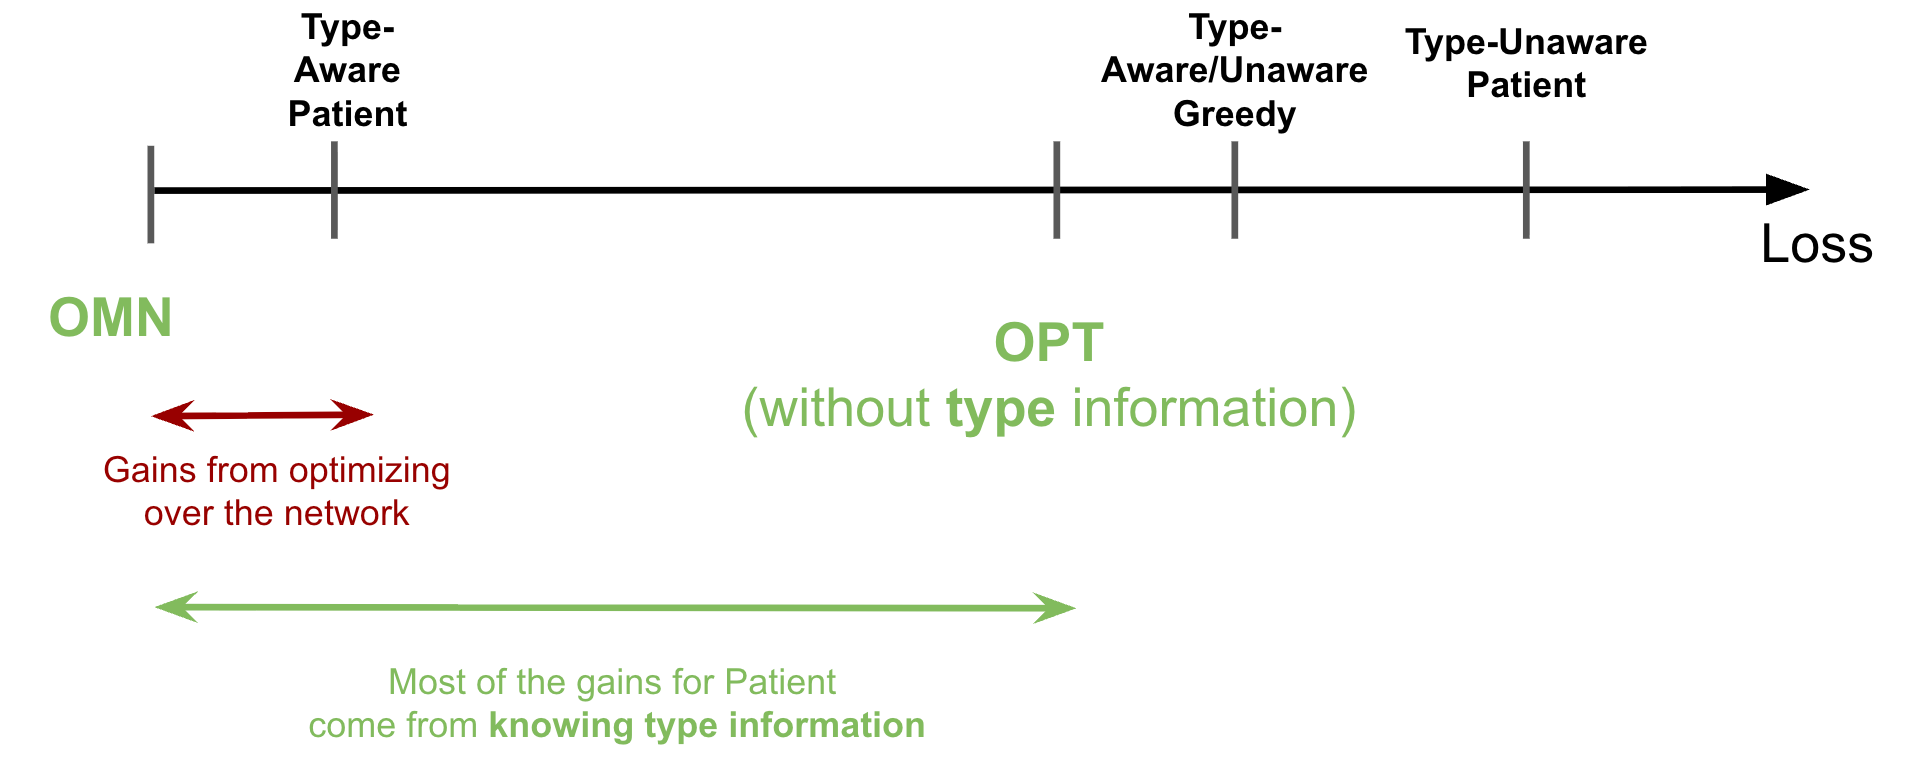
\includegraphics[width=\textwidth]{figures/conjecture.png}
\caption{Qualitative loss ordering suggested by the ODE asymptotics. Moving left means lower loss. The residual gap between the omniscient benchmark and \textbf{TA-Patient} is the gain from full network optimization, while the larger gap to type-unaware \textbf{Patient} reflects the value of type information.}
\label{fig:main-takeaway-ordering}
\end{figure}

\paragraph{Why ODEs appear.}
The original object is a finite stochastic matching market, a continuous-time Markov chain tracking the pool counts $(H_t,E_t)$. In the large-market limit $m\to\infty$, the rescaled pool $(H_t/m,E_t/m)$ has deterministic first-order dynamics: arrivals, criticalities, and matches produce an ODE for the pair $(x(t),y(t))$. The right-hand side of this ODE is the \emph{drift}: the expected infinitesimal net change of the rescaled H and E pools. A fixed point is a state $(x^\ast,y^\ast)$ where both drift coordinates are zero, so H and E inflows, matches, and unmatched criticalities balance on average. Fixed points therefore predict the typical long-run pool composition, and substituting them into the unmatched-criticality rates gives the loss formulas. The computations below come in two layers: ODE fixed-point calculations for the large-market limit, and finite-$m$ CTMC simulations as a direct stochastic check.

\paragraph{Why the homogeneous proof does not transfer verbatim.}
In the one-type model of \cite{akbarpour}, the scalar pool size admits a reduced balance equation and a one-dimensional concentration argument. Here the state is $(H_t,E_t)$, stationary balance is genuinely two-dimensional, and the chain is generally not reversible or product-form; hence ODE fixed points identify candidate concentration points, but converting them into long-run CTMC losses requires the additional stationary-concentration step isolated later as Hypothesis~H.

\section{Experiments}\label{sec:experiments}

\open Figure~\ref{fig:ctmc-perishing-combined} is a finite-market CTMC simulation rather than a proof. We simulate the literal market dynamics with $m=10000$, $d_1=10$, horizon $T=100$, and five independent runs for each policy and each $d_2\in\{10,100,1000,10000\}$. The plotted quantity is cumulative perishing by time $t$, normalized by the common denominator $mT$; shaded regions are mean $\pm$ one standard deviation across runs. The top row aggregates H and E perishing, while the next two rows decompose the same loss by type.

\begin{figure}[p]
\centering
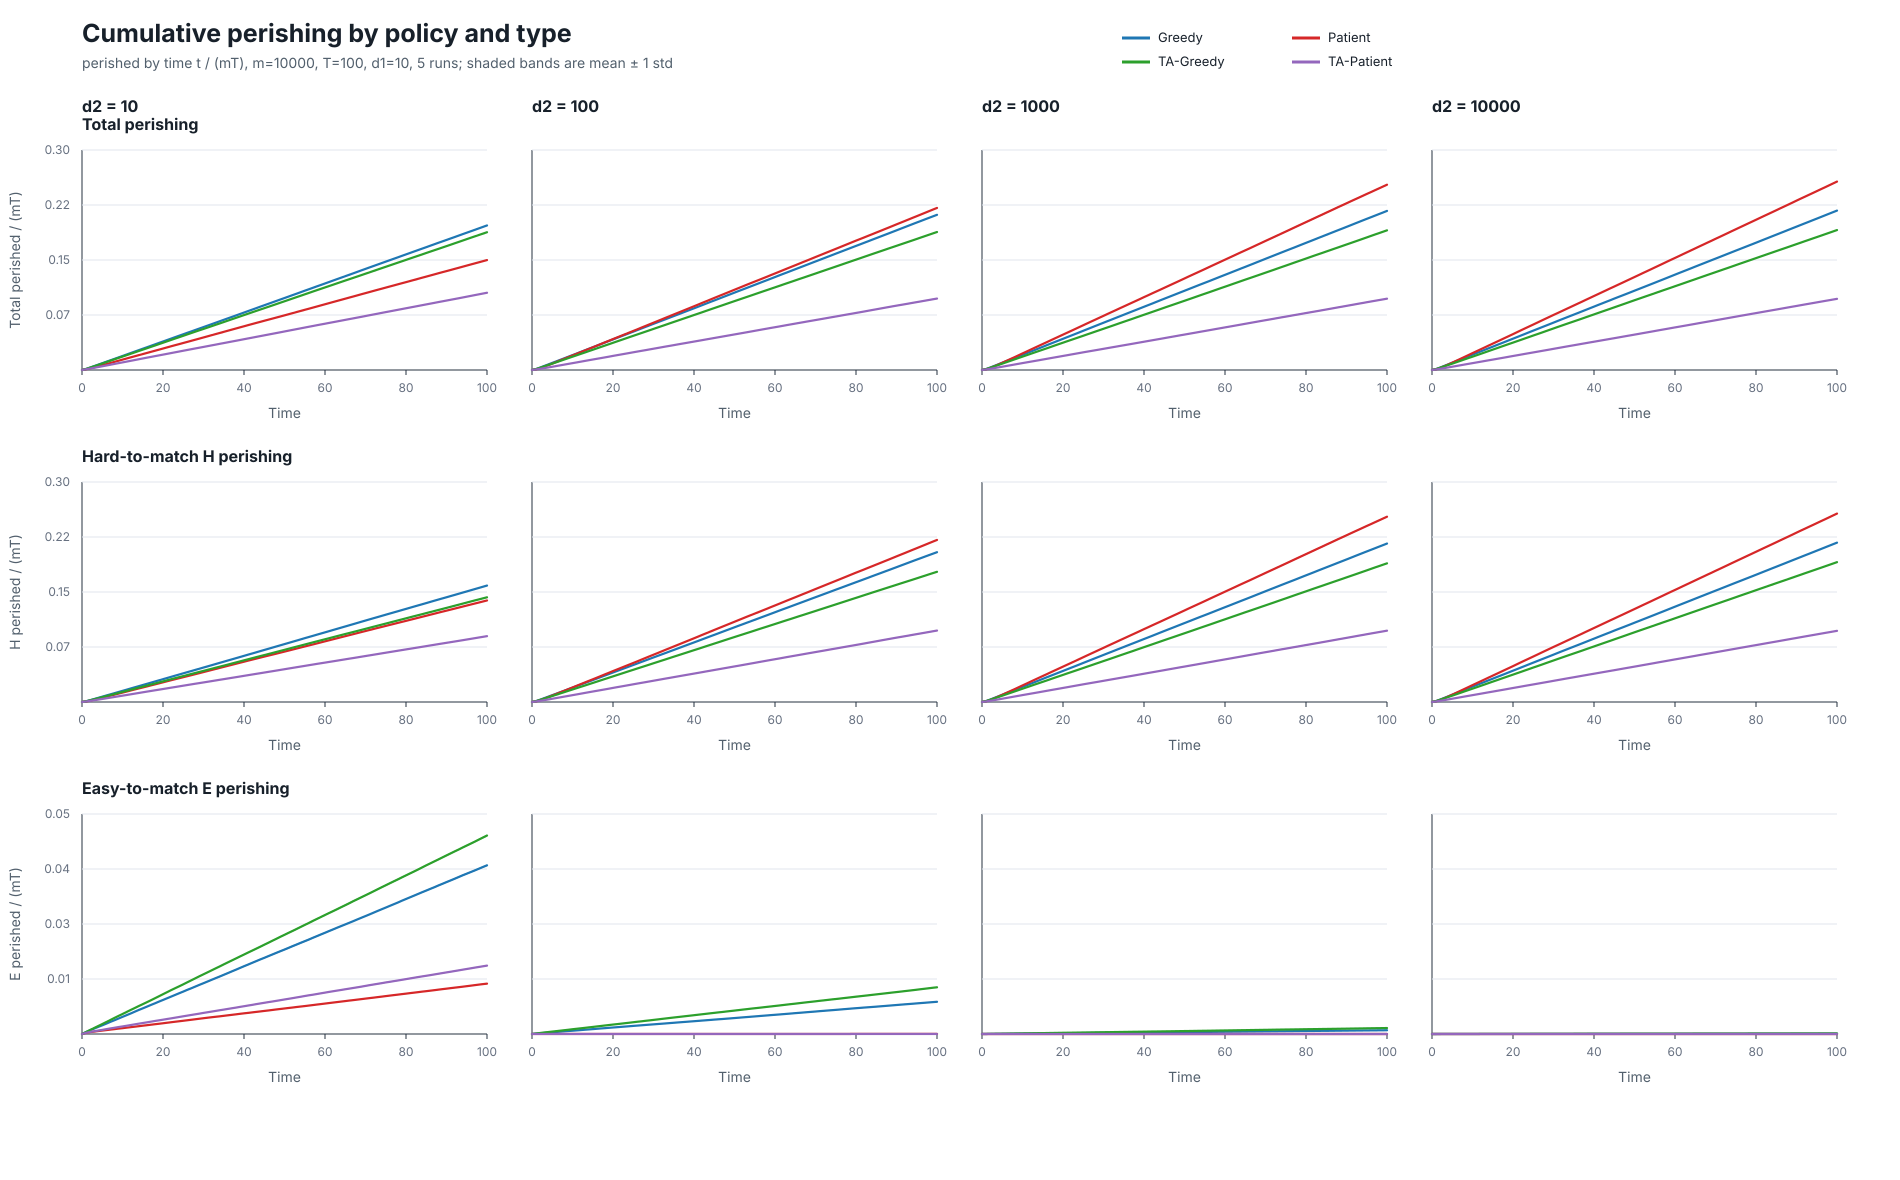
\includegraphics[width=\textwidth]{simulation_outputs/all_perishing_combined_m10000_d1_10_d2_10_100_1000_10000_t100_runs5.png}
\caption{Finite-$m$ CTMC perishing trajectories under the four policies. At mild heterogeneity ($d_2=10$), plain \textbf{Patient} improves on plain \textbf{Greedy}. As the E--E channel strengthens, this ordering reverses: \textbf{Patient}'s loss becomes dominated by H perishing, while \textbf{Greedy} benefits from the thin E pool created by immediate matching. The type-aware rules separate sharply from their plain counterparts; the \textbf{TA-Patient} loss remains lowest throughout and changes little as $d_2$ increases on this grid.}
\label{fig:ctmc-perishing-combined}
\end{figure}

The reversal is visible already in the total-loss row. For $d_2=10$, waiting helps: \textbf{Patient} lies below \textbf{Greedy}. For $d_2\ge 100$, waiting without type-aware selection hurts: \textbf{Patient} rises above \textbf{Greedy}, and the type decomposition shows that the additional loss is almost entirely H perishing. This is the finite-market counterpart of the main mechanism in the ODE analysis: as E--E compatibility becomes abundant, plain Patient spends E criticalities on E partners, whereas type-aware Patient deliberately reserves E opportunities to rescue H agents. The weak dependence of \textbf{TA-Patient} on $d_2$ is also intuitive: once E--E compatibility is plentiful, the binding constraint for rescuing H agents is no longer the E--E channel $d_2$, but the H--E rescue channel governed by $d_1$.

\subsection{Computational evidence (through ODEs)}

\open The next tables are numerical evidence rather than proof. They are placed before the derivations because they are the quickest way to see the policy ranking and the finite-$d_2$ effects. The first three tables are ODE fixed-point computations; the final table is a literal finite-$m$ CTMC simulation.

\paragraph{$d_2=\infty$ ODE fixed points.}
The $d_2=\infty$ fixed-point values are ODE-limit values, with $m\to\infty$ taken first:
\begin{center}
\begin{tabular}{r|cccc}
$d_1$ & $L^{\text{Greedy}}$ & $L^{\text{TA-Greedy}}$ & $L^{\text{Patient}}$ & $L^{\text{TA-Patient}}$\\\hline
$0.5$ & $0.460$ & $0.447$ & $0.471$ & $0.444$\\
$1$   & $0.428$ & $0.408$ & $0.447$ & $0.397$\\
$2$   & $0.379$ & $0.352$ & $0.408$ & $0.325$\\
$5$   & $0.291$ & $0.261$ & $0.331$ & $0.196$\\
$10$  & $0.219$ & $0.192$ & $0.261$ & $9.7\!\times\!10^{-2}$\\
$50$  & $0.088$ & $0.076$ & $0.117$ & $6.8\!\times\!10^{-4}$\\
$100$ & $0.055$ & $0.047$ & $0.076$ & $1.3\!\times\!10^{-6}$
\end{tabular}
\end{center}
These values support the $d_2=\infty$ ordering
\[
L^{\text{TA-Patient}}<L^{\text{TA-Greedy}}\sim L^{\text{Greedy}}<L^{\text{Patient}}
\]
at the leading large-$d_1$ scale. On the displayed grid TA-Greedy is slightly below Greedy, but the two Greedy variants have the same leading asymptotic order; the strict global inequalities remain open analytically.

\paragraph{Joint finite-$(d_1,d_2)$ ODE fixed points.}
The finite-$(d_1,d_2)$ fixed-point table is:
\begin{center}
\begin{tabular}{r|r|ccccc}
Policy & $d_1\backslash d_2$ & $10$ & $50$ & $100$ & $500$ & $\infty$\\\hline
\textbf{Greedy} & $1$  & $0.490$ & $0.444$ & $0.437$ & $0.430$ & $0.428$\\
                & $5$  & $0.292$ & $0.290$ & $0.290$ & $0.291$ & $0.291$\\
                & $10$ & $0.198$ & $0.209$ & $0.213$ & $0.217$ & $0.219$\\\hline
\textbf{TA-Greedy} & $1$  & $0.480$ & $0.428$ & $0.418$ & $0.410$ & $0.408$\\
                   & $5$  & $0.280$ & $0.266$ & $0.264$ & $0.261$ & $0.261$\\\hline
\textbf{Patient} & $1$  & $0.466$ & $0.438$ & $0.442$ & $0.446$ & $0.447$\\
                 & $5$  & $0.259$ & $0.293$ & $0.309$ & $0.326$ & $0.331$\\\hline
\textbf{TA-Patient} & $1$  & $0.443$ & $0.398$ & $0.397$ & $0.397$ & $0.397$\\
                    & $5$  & $0.214$ & $0.197$ & $0.196$ & $0.196$ & $0.196$
\end{tabular}
\end{center}
Here the $\infty$ column is the same sequential ODE limit as above, not a finite-$m$ simulation. \textbf{TA-Patient} reaches its asymptotic value to three decimal places by $d_2=100$ in the displayed rows; the other policies show visible algebraic $1/d_2$ effects.

\paragraph{Greedy-vs-Patient crossover.}
At $d_1=1$, the Greedy-vs-Patient comparison flips between $d_2=50$ and $d_2=70$:
\begin{center}
\begin{tabular}{r|ccccccccc}
$d_2$               & 5 & 10 & 20 & 30 & 50 & 70 & 100 & 200 & 500\\\hline
$L^{\text{Greedy}}$  & $0.525$ & $0.490$ & $0.464$ & $0.454$ & $0.444$ & $0.440$ & $0.437$ & $0.432$ & $0.430$\\
$L^{\text{Patient}}$ & $0.506$ & $0.466$ & $0.442$ & $0.437$ & $0.438$ & $0.440$ & $0.442$ & $0.445$ & $0.446$\\
winner               & P & P & P & P & P & G & G & G & G
\end{tabular}
\end{center}
This is the formal counterpart of the empirical pattern reported by \cite{Liu2019TheEO}: when type heterogeneity is mild, waiting helps; when pronounced, waiting hurts.

\paragraph{Finite-$m$ CTMC simulation.}
We ran literal finite-$m$ CTMC simulations of all four policies with $m=5000$ and $m=10000$, $n_{\mathrm{runs}}=3$, burn-in time $10$, and horizon $80$. These are finite-$m$, finite-$d_2$ simulations; the $d_2=\infty$ values elsewhere are sequential ODE limits, not simulations.
\begin{center}
{\small
\begin{tabular}{rrr|r|ccc}
$m$ & $d_1$ & $d_2$ & Policy & ODE loss & CTMC loss & Gap\\\hline
$5000$  & $1$ & $50$  & Greedy     & $0.4443$ & $0.4440\pm0.0004$ & $0.0004$\\
$5000$  & $1$ & $50$  & Patient    & $0.4382$ & $0.4380\pm0.0004$ & $0.0002$\\
$5000$  & $1$ & $50$  & TA-Greedy  & $0.4275$ & $0.4277\pm0.0001$ & $0.0003$\\
$5000$  & $1$ & $50$  & TA-Patient & $0.3976$ & $0.3979\pm0.0009$ & $0.0003$\\
$5000$  & $5$ & $100$ & Greedy     & $0.2902$ & $0.2900\pm0.0006$ & $0.0002$\\
$5000$  & $5$ & $100$ & Patient    & $0.3088$ & $0.3087\pm0.0007$ & $0.0002$\\
$5000$  & $5$ & $100$ & TA-Greedy  & $0.2637$ & $0.2630\pm0.0005$ & $0.0007$\\
$5000$  & $5$ & $100$ & TA-Patient & $0.1963$ & $0.1969\pm0.0005$ & $0.0006$\\
$10000$ & $1$ & $50$  & Greedy     & $0.4443$ & $0.4442\pm0.0002$ & $0.0001$\\
$10000$ & $1$ & $50$  & Patient    & $0.4382$ & $0.4382\pm0.0010$ & $0.0001$\\
$10000$ & $1$ & $50$  & TA-Greedy  & $0.4275$ & $0.4281\pm0.0006$ & $0.0006$\\
$10000$ & $1$ & $50$  & TA-Patient & $0.3976$ & $0.3978\pm0.0010$ & $0.0002$\\
$10000$ & $5$ & $100$ & Greedy     & $0.2902$ & $0.2896\pm0.0001$ & $0.0005$\\
$10000$ & $5$ & $100$ & Patient    & $0.3088$ & $0.3086\pm0.0009$ & $0.0003$\\
$10000$ & $5$ & $100$ & TA-Greedy  & $0.2637$ & $0.2644\pm0.0003$ & $0.0007$\\
$10000$ & $5$ & $100$ & TA-Patient & $0.1963$ & $0.1963\pm0.0008$ & $0.0001$
\end{tabular}
}
\end{center}
The simulations are not a proof of Hypothesis~H, but they are consistent with the ODE fixed-point predictions at the tested parameters.

The rest of the paper derives the ODE fixed-point formulas behind this separation and then records the precise assumptions needed to interpret the formulas as stochastic long-run losses.


\section{Main Results and Standing Hypothesis}
\label{sec:main}

\subsection{Setup and notation}

The pool state is $(H_t,E_t)\in\mathbb{Z}_{\ge 0}^2$. The rescaled process is $X^m_t=(H^m_t,E^m_t)/m\in\mathbb{R}_+^2$ (state space unbounded; counts have $\mathrm{Poisson}(m)$ tails). All asymptotics are sequential: $m\to\infty$ first, then $d_2\to\infty$ with $d_1$ fixed. The first limit gives the mean-field ODE; the second gives the limiting fixed-point formulas below. Thus a displayed $d_2=\infty$ value means $\lim_{d_2\to\infty}\lim_{m\to\infty}$ at the ODE fixed point, not a finite-$m$ CTMC simulation with infinite compatibility probability.

In large-$d_1$ statements we suppress constants inside logarithms when only the leading asymptotic is being reported: for any fixed $c>0$, $\log(d_1/c)\sim\log d_1$.

Throughout the ODE analysis, $\pi_H(x,y)$ and $\pi_E(x,y)$ denote \emph{compatibility-availability probabilities}, not stationary distributions. At a scaled pool state $(x,y)$,
\[
\pi_H(x,y)=1-e^{-d_1y/2},\qquad
\pi_E(x,y)=1-e^{-(d_1x+d_2y)/2}.
\]
Thus $\pi_H$ is the probability that an H agent facing the pool sees at least one compatible E, and $\pi_E$ is the probability that an E agent sees at least one compatible H or E. The stationary distribution of the finite CTMC is denoted separately by $\pi_m$.

For the plain uniform-among-neighbours policies, $\rho_{i\to j}$ denotes the conditional share of matched partners of type $j$ when the active agent has type $i$ and has at least one compatible neighbour. Since H can only match E,
\[
\rho_{H\to E}(x,y)=1.
\]
For an E agent, the fluid neighbour intensities are $d_1x/2$ for H neighbours and $d_2y/2$ for E neighbours, so whenever $d_1x+d_2y>0$,
\[
\rho_{E\to H}(x,y)=\frac{d_1x}{d_1x+d_2y},\qquad
\rho_{E\to E}(x,y)=\frac{d_2y}{d_1x+d_2y}.
\]
At $(x,y)=(0,0)$ the conditional shares are immaterial because $\pi_E(0,0)=0$; we set the products $\pi_E\rho_{E\to H}$ and $\pi_E\rho_{E\to E}$ to $0$ there. For compactness we write
\[
r_{EH}:=\pi_E\rho_{E\to H},\qquad r_{EE}:=\pi_E\rho_{E\to E}.
\]

\subsection{Hypothesis~H (stationary concentration)}\label{ssec:hypH}

\open
We assume that for each policy and each $(d_1,d_2)$, the unique stationary distribution $\pi_m$ of $X^m_t$ (Lemma~\ref{lem:stationary}) concentrates as $m\to\infty$:
\[
\pi_m \;\Longrightarrow\; \delta_{(x^\ast,y^\ast)},
\]
where $(x^\ast,y^\ast)\in\mathbb{R}_+^2$ is the relevant selected zero of the policy-specific limiting drift. This bundles three sub-claims, none proved here: global attraction or branch selection for $(x^\ast,y^\ast)$ in the ODE; tightness of $\{\pi_m\}$; interchange of limits $\lim_{t\to\infty}\lim_{m\to\infty}=\lim_{m\to\infty}\lim_{t\to\infty}$. A plausible proof route is an Akbarpour--Li--Oveis Gharan style coupling argument \cite{akbarpour}, but the coupling has to be more nuanced here: it must track both H and E counts and the type of the removed partner, not just the total pool size. The hypothesis is supported by numerics but is not used to prove the deterministic fixed-point formulas; its role is to transfer those formulas to long-run CTMC losses.


\subsection{Standalone ODE loss theorems as $d_2\to\infty$}\label{ssec:results-d2inf}

The next three theorems are the fully proved ODE fixed-point loss formulas. They are ODE-level statements: interpreting them as long-run CTMC loss formulas additionally requires Hypothesis~H.

\begin{theorem}[Greedy ODE fixed point and loss]\label{thm:greedy-ode-loss}
\proved For every $d_1>0$, in the limit $m\to\infty$ followed by $d_2\to\infty$, the Greedy ODE fixed point satisfies
\[
(x^\star_G(d_1),y^\star_G(d_1))=(x^\star_G(d_1),0),
\]
where $x^\star_G(d_1)$ is the unique root in $(0,1/2)$ of
\[
x\,\exp\!\left(\frac{d_1\,x(1-x)}{2(1-2x)}\right)=1.
\]
Equivalently, along the finite-$d_2$ branch,
\[
y^\star_G(d_1,d_2)=\frac{1}{d_2}\frac{d_1(x^\star_G)^2}{1-2x^\star_G}+O(d_2^{-2}).
\]
The corresponding loss is
\begin{equation}\label{eq:LG}
L^{\text{Greedy}}(d_1) \;=\; x^\star_G(d_1).
\end{equation}
As $d_1\to\infty$,
\[
x^\star_G(d_1)
\sim \frac{2W(d_1/2)}{d_1}
\sim \frac{2\log d_1}{d_1}.
\]
The Lambert-$W$ expression here is an asymptotic approximation, not an exact closed form.
\end{theorem}

\begin{proof}
Lemma~\ref{lem:greedy-scalar} proves that Greedy fixed points have $y=O(1/d_2)$, reduce to the displayed scalar equation, and have a unique root in $(0,1/2)$. For the large-$d_1$ approximation, the root must tend to $0$; otherwise the exponent diverges and the scalar equation cannot hold. Thus the equation reduces at leading order to $x\exp(d_1x/2)=1$, and a standard monotonicity perturbation around this leading equation gives $x\sim 2W(d_1/2)/d_1$. Finally $W(z)\sim\log z$ gives the stated logarithmic scale.
\end{proof}

\begin{theorem}[Type-Aware Greedy ODE fixed point and loss]\label{thm:tag-ode-loss}
\proved For every $d_1>0$, in the limit $m\to\infty$ followed by $d_2\to\infty$, the Type-Aware Greedy ODE fixed point is
\[
(x^\star_{TAG}(d_1),y^\star_{TAG}(d_1))
=
\left(\frac{2W(d_1/4)}{d_1},\,0\right).
\]
Equivalently, along the finite-$d_2$ branch,
\[
y^\star_{TAG}(d_1,d_2)=\frac{2\log 2}{d_2}+O(d_2^{-2}).
\]
The corresponding loss is
\begin{equation}\label{eq:LTG}
L^{\text{TA-Greedy}}(d_1) \;=\; \frac{2\,W(d_1/4)}{d_1}.
\end{equation}
As $d_1\to\infty$,
\[
x^\star_{TAG}(d_1)=L^{\text{TA-Greedy}}(d_1)
\sim \frac{2\log d_1}{d_1}.
\]
\end{theorem}

\begin{proof}
Lemma~\ref{lem:TAG} proves that the $d_2\to\infty$ fixed point has $y=O(1/d_2)$ and limiting $x$ satisfying $2x=e^{-d_1x/2}$, equivalently $x=2W(d_1/4)/d_1$. The large-$d_1$ asymptotic follows from $W(z)\sim\log z$.
\end{proof}

\begin{theorem}[Patient ODE fixed point and loss]\label{thm:patient-ode-loss}
\proved For every $d_1>0$, in the limit $m\to\infty$ followed by $d_2\to\infty$, the Patient ODE fixed point is
\[
(x^\star_P(d_1),y^\star_P(d_1))
=
\left(\frac12,\,\frac{2W(d_1/8)}{d_1}\right).
\]
The corresponding loss is
\begin{equation}\label{eq:LP}
L^{\text{Patient}}(d_1) \;=\; \frac{4\,W(d_1/8)}{d_1}.
\end{equation}
As $d_1\to\infty$,
\[
y^\star_P(d_1)\sim \frac{2\log d_1}{d_1},
\qquad
L^{\text{Patient}}(d_1)\sim \frac{4\log d_1}{d_1}.
\]
\end{theorem}

\begin{proof}
Lemma~\ref{lem:Patient} proves that Patient fixed points satisfy $x\to1/2$ and $y\to y^\ast(d_1)$ with $e^{-d_1y^\ast/2}=4y^\ast$, so $y^\ast=2W(d_1/8)/d_1$ and the aggregate loss is $2y^\ast$. The large-$d_1$ asymptotic again follows from $W(z)\sim\log z$.
\end{proof}

\paragraph{TA-Patient status.}
\open For every $d_1>0$, the $d_2=\infty$ limiting system \eqref{eq:TAP1}--\eqref{eq:TAP2} has a solution $(x^\ast,y^\ast)$ along which
\begin{equation}
L^{\text{TA-Patient}}(d_1) \;=\; x^\ast(d_1)\,e^{-d_1\,y^\ast(d_1)/2}.\label{eq:LTP}
\end{equation}
Existence is by Poincar\'e--Miranda; uniqueness is open. Lemma~\ref{lem:TAP} gives a formal local branch near $(1/4,1/4)$ for large $d_1$, conditional on the stated local non-degeneracy, along which
\[
L^{\text{TA-Patient}}(d_1) \;\sim\; \frac{\sqrt{2}}{4}\,e^{-d_1/8}\qquad(d_1\to\infty).
\]
For the displayed parameter grid, the fixed-point solver and multi-start root scan found a single admissible TA-Patient root. This is only numerical evidence for the selected branch in those cases, not a proof of global uniqueness.

\subsection{Patient $\leftrightarrow$ TA-Greedy duality}

\proved The closed forms \eqref{eq:LTG}, \eqref{eq:LP} satisfy
\[
L^{\text{Patient}}(d_1) \;=\; L^{\text{TA-Greedy}}(d_1/2).
\]
Plain \textbf{Patient} at H-E density $d_1$ matches \textbf{TA-Greedy} at half that density: the two policies trade compatibility density for type information at a 2-to-1 rate.

\section{The Pool Process}
\label{sec:markov}

\paragraph{Finite-count compatibility probabilities.}
The finite CTMC uses the same notation with count arguments. For an agent facing pool $(h,e)$, independence across pairs gives
\begin{equation}\label{eq:pi}
\pi_H(h,e)=1-(1-p_{HE})^e,\qquad \pi_E(h,e)=1-(1-p_{HE})^h(1-p_{EE})^e.
\end{equation}
Here $\pi_H(h,e)$ is the probability that an H agent sees at least one compatible E, and $\pi_E(h,e)$ is the probability that an E agent sees at least one compatible H or E. The function $\pi_H$ has no $h$-dependence because $p_{HH}=0$. For a critical E already inside the pool, the finite-count E--E term uses $e-1$ rather than $e$ to exclude self-matching; this changes the formulas by $O(1/m)$ and disappears in the fluid limit. If $h/m\to x$ and $e/m\to y$, then \eqref{eq:pi} converges to the fluid probabilities defined in the Setup section.

\begin{lemma}[Poisson neighbour limits]\label{lem:poisson-neighbour}
\proved Suppose $h_m/m\to x$ and $e_m/m\to y$ while $p_{HE}=d_1/(2m)$ and $p_{EE}=d_2/(2m)$. For an H agent facing the pool,
\[
N_{HE}\sim \mathrm{Bin}(e_m,p_{HE})
\quad\Longrightarrow\quad
\mathrm{Poisson}(d_1y/2).
\]
For an E agent facing the pool,
\[
N_{EH}\sim \mathrm{Bin}(h_m,p_{HE}),\qquad
N_{EE}\sim \mathrm{Bin}(e_m,p_{EE})
\]
are independent for each $m$ (with $e_m-1$ in place of $e_m$ for a critical E already in the pool, giving the same limit), and jointly
\[
(N_{EH},N_{EE})
\quad\Longrightarrow\quad
\bigl(\mathrm{Poisson}(d_1x/2),\,\mathrm{Poisson}(d_2y/2)\bigr),
\]
with independent limiting coordinates.
\end{lemma}

\begin{proof}
For $N_{EH}$, the probability generating function is
\[
\E[s^{N_{EH}}]
=\left(1+\frac{d_1(s-1)}{2m}\right)^{h_m}
\;\longrightarrow\;
\exp\!\left(\frac{d_1x}{2}(s-1)\right),
\]
the pgf of $\mathrm{Poisson}(d_1x/2)$. The same calculation gives $N_{HE}\Rightarrow\mathrm{Poisson}(d_1y/2)$ and $N_{EE}\Rightarrow\mathrm{Poisson}(d_2y/2)$. Since $N_{EH}$ and $N_{EE}$ are independent for every finite $m$, their joint pgf factors for every $m$ and the limiting joint pgf is the product of the two Poisson pgfs. Hence the limits are independent.
\end{proof}

\paragraph{Selection rules.}
Both selection rules are local: the policy only observes the current agent's compatible neighbours in the pool. The difference is tie-breaking. Plain Greedy/Patient chooses uniformly among compatible neighbours, while the type-aware variants first ask whether any compatible H neighbour is available and choose H before E.

Let $N_{HE}\sim\mathrm{Bin}(e,p_{HE})$ be the number of E neighbours seen by an H agent, and let $N_{EH}\sim\mathrm{Bin}(h,p_{HE})$ and $N_{EE}\sim\mathrm{Bin}(e,p_{EE})$ be the independent H- and E-neighbour counts seen by an E agent. For a critical E, replace $e$ by $e-1$ in $N_{EE}$ at finite $m$; the limiting expressions are unchanged. The \emph{uniform-among-neighbours} rule (used by plain Greedy/Patient) has $\rho_{H\to E}=1$ on $\{N_{HE}\ge 1\}$ and
\[
\rho_{E\to H}(h,e)=\E\!\left[\frac{N_{EH}}{N_{EH}+N_{EE}}\,\bigg|\,N_{EH}+N_{EE}>0\right],\qquad \rho_{E\to E}=1-\rho_{E\to H}.
\]
The \emph{H-priority} rule (used by Type-Aware Greedy/Patient) has $\widetilde\rho_{H\to E}=1$ on $\{N_{HE}\ge 1\}$, and for E:
\[
\pi_E\,\widetilde\rho_{E\to H}=1-(1-p_{HE})^h,\qquad \pi_E\,\widetilde\rho_{E\to E}=(1-p_{HE})^h\bigl(1-(1-p_{EE})^e\bigr).
\]
The two right-hand sides sum to $\pi_E$, as they should.

\begin{lemma}[Conditional pool law]\label{lem:pool}
\proved Let $\mathcal{G}_t$ be the event-and-revelation filtration: arrivals, criticalities, matching decisions, and edge variables they reveal. Then conditional on $\mathcal{G}_t$ with $(H_t,E_t)=(h,e)$:
\begin{enumerate}
\item Under any \textbf{Greedy} variant, the pool graph is almost surely edgeless.
\item Under any \textbf{Patient} variant, the unrevealed edges among pooled agents are independent with the probabilities of \eqref{eq:regime}.
\end{enumerate}
The transition probabilities of $(H_t,E_t)$ depend only on $(h,e)$, so $(H_t,E_t)$ is a CTMC.
\end{lemma}

\begin{proof}
\emph{Greedy.} Suppose two pooled agents $a,b$ with arrival times $s_a<s_b$ had a compatible edge. At time $s_b$, agent $b$ would have matched (with $a$ or earlier), contradicting both being still pooled.

\emph{Patient (deferred decision).} Build the model carrying independent Bernoullis $\{\xi_{\{i,j\}}\sim\mathrm{Bernoulli}(p_{\tau_i\tau_j})\}$ over unordered pairs of agents. Edge $\{i,j\}$ exists iff $\xi_{\{i,j\}}=1$. A pair is \emph{revealed} the first time a matching decision tests it. Inductive claim: at every event time, unrevealed Bernoullis are conditionally independent given $\mathcal{G}_t$ with their original marginals. Base case: trivial at $t=0$. Step: an arrival reveals nothing under Patient. A criticality of $a$ reveals $\{\xi_{\{a,i\}}:i\text{ pooled}\}$, which by hypothesis are independent of unrevealed pairs not incident on $a$; the policy's choice of partner is a function of the revealed values; after $a$ (and possibly its partner) leave, the pairs incident on them are no longer relevant, and the remaining unrevealed structure is unchanged. The Markov property follows: rates depend only on counts.
\end{proof}

\begin{lemma}[Stationarity]\label{lem:stationary}
\proved Under any policy, $(H_t,E_t)$ is irreducible, nonexplosive, and has a unique stationary distribution.
\end{lemma}

\begin{proof}
Take Lyapunov $V(h,e)=h+e$. The CTMC generator gives $\mathcal A V\le m-(h+e)$: arrivals contribute $+m$ total; criticalities and matchings contribute at least $-(h+e)$. So $\mathcal A V<0$ outside $\{h+e\le m\}$, and Foster--Lyapunov \cite[Theorem~5.5]{meyn1993stability} gives positive recurrence. The total event rate at $(h,e)$ is at most $m+(h+e)$, linear in the state, so the chain is nonexplosive. Irreducibility: from any state, with positive probability no arrivals occur before the pool empties; each criticality firing removes at least one agent, so the chain reaches $(0,0)$ after finitely many such firings. Conversely, $(0,0)$ reaches any target state via a finite sequence of arrivals before any criticality clock fires, with compatibility draws returning $0$ against all previously pooled agents; this event has positive probability.
\end{proof}

\paragraph{Mixing time (open).}
\open Lemma~\ref{lem:stationary} gives stationarity for each finite $m$, but not a quantitative approach rate. To use stationary ODE losses as finite-horizon CTMC predictions, one needs $t_{\mathrm{mix}}(m,d_1,d_2)=o(T)$ on the relevant horizon $T$, together with the stationary concentration in Hypothesis~H. The Lyapunov calculation above proves recurrence; it does not give a useful uniform-in-$m$ mixing bound. We conjecture $t_{\mathrm{mix}}=O(\log m)$ for fixed $(d_1,d_2)$, with constants possibly growing in $d_2$. A proof should likely adapt the homogeneous-model coupling of \cite{akbarpour}, but here the coupling must control the full vector $(H,E)$: two chains can have the same total pool size while having different type composition, and composition changes future H--E and E--E match probabilities.


\section{Mean-Field Analysis under Greedy}
\label{sec:greedy}

\subsection{Fluid-limit drift and Kurtz convergence}\label{ssec:greedy-drift}

The fluid limit uses standard density-dependent Markov-chain notation. A jump vector $v=(1,0)$ means the count process $(H,E)$ increases by one H; in the rescaled process $X^m=(H,E)/m$, the same transition has size $v/m$. The symbol $\beta_v$ has one input: the current scaled state vector $z\in\mathbb R_+^2$. When $z=(x,y)$, we write either $\beta_v(z)$ or, as shorthand, $\beta_v(x,y)$. It is the \emph{rate density} of jump $v$ at that state: the actual CTMC transition rate is
\[
\text{rate}\{X^m\to X^m+v/m\}\;=\;m\,\beta_v(z)+o(m).
\]
Thus $\beta_v$ is not a probability. It is the order-$m$ rate divided by $m$. Multiplying jump size by jump rate gives
\[
\frac{v}{m}\cdot m\beta_v(z)=v\,\beta_v(z),
\]
which is why the ODE drift is $F(z)=\sum_v v\,\beta_v(z)$.

At a scaled state $(x,y)$, a new H agent sees at least one compatible E with probability
\[
\pi_H(x,y)=1-e^{-d_1y/2},
\]
while a new or critical E agent sees at least one compatible pooled neighbour with probability
\[
\pi_E(x,y)=1-e^{-(d_1x+d_2y)/2}.
\]
By Lemma~\ref{lem:poisson-neighbour}, the H-neighbour and E-neighbour intensities seen by an E agent are $d_1x/2$ and $d_2y/2$ in the fluid limit. Conditional on seeing some neighbour, the fluid share assigned to H is $d_1x/(d_1x+d_2y)$ and the share assigned to E is $d_2y/(d_1x+d_2y)$. Thus the unconditional probabilities that an E event selects an H or an E partner are
\begin{align*}
r_{EH}(x,y) &= \bigl(1-e^{-(d_1 x+d_2 y)/2}\bigr)\,\frac{d_1 x}{d_1 x+d_2 y},\\
r_{EE}(x,y) &= \bigl(1-e^{-(d_1 x+d_2 y)/2}\bigr)\,\frac{d_2 y}{d_1 x+d_2 y},
\end{align*}
both extended by $0$ at the origin and Lipschitz on every compact subset of $\mathbb{R}_+^2$. (For type-aware policies, replace $r_{EH}$ by $\widetilde r_{EH}=1-e^{-d_1 x/2}$ and $r_{EE}$ by $\widetilde r_{EE}=e^{-d_1 x/2}(1-e^{-d_2 y/2})$, both smooth.)

\paragraph{Plain Greedy rate accounting.}
Under Greedy, matching decisions occur only at arrivals. If an arriving agent matches, the arrival itself never joins the pool; only its chosen pooled partner is removed. Also, by Lemma~\ref{lem:pool}, the Greedy pool is edgeless, so a pooled agent that becomes critical has no compatible neighbour left in the pool and simply leaves unmatched.

Hence the possible scaled jumps are $\mathcal V=\{\pm e_1,\pm e_2\}$:
\begin{align*}
\beta_{(1,0)}&=\tfrac12(1-\pi_H),
&\beta_{(0,1)}&=\tfrac12(1-\pi_E),\\
\beta_{(-1,0)}&=x+\tfrac12 r_{EH},
&\beta_{(0,-1)}&=y+\tfrac12\pi_H+\tfrac12 r_{EE}.
\end{align*}
The first row is the unmatched-arrival inflow: an H arrival joins only if it sees no E, and an E arrival joins only if it sees no compatible neighbour. The second row is outflow from the existing pool: H criticalities remove H at rate $x$, E arrivals that choose H remove H at rate $\tfrac12r_{EH}$, E criticalities remove E at rate $y$, H arrivals that match remove E at rate $\tfrac12\pi_H$, and E arrivals that choose E remove E at rate $\tfrac12r_{EE}$.

Component-wise, if $X_H=H/m$ and $X_E=E/m$, the $m$'s cancel as follows. For the H coordinate,
\[
\begin{aligned}
\dot X_H
&=\frac{1}{m}\Bigl[
\underbrace{\frac m2(1-\pi_H)}_{\text{unmatched H arrivals}}
-\underbrace{mx}_{\text{H criticalities}}
-\underbrace{\frac m2 r_{EH}}_{\text{E arrivals choosing H}}
\Bigr]\\
&=\tfrac12(1-\pi_H)-x-\tfrac12 r_{EH}.
\end{aligned}
\]
For the E coordinate,
\[
\begin{aligned}
\dot X_E
&=\frac{1}{m}\Bigl[
\underbrace{\frac m2(1-\pi_E)}_{\text{unmatched E arrivals}}
-\underbrace{my}_{\text{E criticalities}}
-\underbrace{\frac m2\pi_H}_{\text{H arrivals choosing E}}
-\underbrace{\frac m2 r_{EE}}_{\text{E arrivals choosing E}}
\Bigr]\\
&=\tfrac12(1-\pi_E)-y-\tfrac12\pi_H-\tfrac12 r_{EE}.
\end{aligned}
\]
The displayed ODE drift is exactly these two component balances.

\begin{proposition}[Greedy fluid limit via Kurtz]\label{prop:kurtz}
\proved For any $T<\infty$ and deterministic $X^m_0\to z_0\in\mathbb{R}_+^2$,
\[
\sup_{t\le T}\|X^m_t-z(t)\|\;\longrightarrow 0\text{ in probability,}\qquad m\to\infty,
\]
where $z(t)$ solves $\dot z=F(z):=\sum_v v\,\beta_v(z)$ with $z(0)=z_0$. Fluctuations are $O(1/\sqrt m)$ on intervals where $z(t)$ stays in a compact region \cite[Ch.~11]{ethier_kurtz}.
\end{proposition}

\begin{proof}[Proof sketch]
This is an application of the density-dependent Markov chain theorem of Ethier--Kurtz, not a new fluid-limit theorem. The hypotheses are as follows.

First, the Greedy chain has a finite jump set $\mathcal V=\{\pm e_1,\pm e_2\}$ and each jump of $X^m$ has size $1/m$. Second, if $z=(h/m,e/m)$ remains in a compact set, the finite-$m$ transition-rate densities converge uniformly to the displayed $\beta_v(z)$. For $\pi_H,\pi_E$ this is immediate from
\[
\left(1-\frac{a}{m}\right)^{\lfloor mz\rfloor}\to e^{-az};
\]
for the E-partner selection terms it follows from the same binomial-to-Poisson pgf estimate, uniformly on compact subsets, and the product definitions $r_{EH}=\pi_E\rho_{E\to H}$, $r_{EE}=\pi_E\rho_{E\to E}$, extended continuously at the origin. Third, the limiting drift
\[
F(z)=\sum_{v\in\mathcal V}v\,\beta_v(z)
\]
is locally Lipschitz because $\pi_H,\pi_E,r_{EH},r_{EE}$ are locally Lipschitz on $\mathbb R_+^2$. Finally, compact containment on finite horizons follows from the linear rate bound: arrivals occur at rate at most $m$, while criticalities and matches only decrease the total pool size. Thus, from bounded initial conditions, $H_t+E_t$ is stochastically dominated above by its initial value plus a Poisson process of rate $m$ on any finite time interval. Ethier--Kurtz then gives the stated uniform convergence on $[0,T]$; the $O(1/\sqrt m)$ fluctuation scale is the corresponding martingale scale on compact intervals.
\end{proof}

The Greedy drift in components is
\begin{align}
F_1(x,y) &= \tfrac12(1-\pi_H)-x-\tfrac12 r_{EH},\label{eq:F1}\\
F_2(x,y) &= \tfrac12(1-\pi_E)-y-\tfrac12\pi_H-\tfrac12 r_{EE}.\label{eq:F2}
\end{align}
The same density-dependent-chain verification applies to the other three policies: the jump set remains finite and bounded, the finite-count transition-rate densities converge locally uniformly to the displayed ODE rates, and the same compact-containment estimate controls finite horizons. We spell out Greedy because it contains the only uniform-neighbour dilution terms; the type-aware and Patient variants are obtained by replacing the selection probabilities and/or moving matching events from arrivals to criticalities.

\subsection{Fixed-point system at finite $(d_1,d_2)$}\label{ssec:greedy-fp}

\begin{lemma}[Greedy aggregate balance and imbalance]\label{lem:greedy-aggreg}
\proved Any interior fixed point of \eqref{eq:F1}--\eqref{eq:F2} satisfies
\begin{align}
x^\ast+y^\ast &= 1-\pi_H(x^\ast,y^\ast)-\pi_E(x^\ast,y^\ast),\label{eq:S1}\\
x^\ast-y^\ast &= r_{EE}(x^\ast,y^\ast).\label{eq:S2}
\end{align}
\end{lemma}

\begin{proof}
Set $F_1=F_2=0$. Adding \eqref{eq:F1} and \eqref{eq:F2}:
\[
0\;=\;\tfrac12(1-\pi_H)+\tfrac12(1-\pi_E)-(x+y)-\tfrac12\pi_H-\tfrac12(r_{EH}+r_{EE}).
\]
Now $r_{EH}+r_{EE}=\pi_E\rho_{E\to H}+\pi_E\rho_{E\to E}=\pi_E$ since $\rho_{E\to H}+\rho_{E\to E}=1$. Substituting,
\[
0\;=\;\tfrac12(1-\pi_H)+\tfrac12(1-\pi_E)-(x+y)-\tfrac12\pi_H-\tfrac12\pi_E\;=\;1-\pi_H-\pi_E-(x+y),
\]
which gives \eqref{eq:S1}. Subtracting \eqref{eq:F2} from \eqref{eq:F1}:
\[
0\;=\;\tfrac12(\pi_E-\pi_H)-(x-y)-\tfrac12 r_{EH}+\tfrac12\pi_H+\tfrac12 r_{EE}\;=\;\tfrac12\pi_E-(x-y)-\tfrac12 r_{EH}+\tfrac12 r_{EE},
\]
where the $\pi_H$ terms cancelled. Using $\pi_E=r_{EH}+r_{EE}$, we get $\tfrac12\pi_E-\tfrac12 r_{EH}+\tfrac12 r_{EE}=\tfrac12 r_{EE}+\tfrac12 r_{EE}=r_{EE}$, giving \eqref{eq:S2}.
\end{proof}

In rescaled-degree variables, \eqref{eq:S1}--\eqref{eq:S2} read
\begin{align}
x+y &= e^{-d_1 y/2}+e^{-(d_1 x+d_2 y)/2}-1, \tag{$S_1'$}\label{eq:S1prime}\\
x-y &= \bigl(1-e^{-(d_1 x+d_2 y)/2}\bigr)\,\frac{d_2 y}{d_1 x+d_2 y}. \tag{$S_2'$}\label{eq:S2prime}
\end{align}

\begin{lemma}[Existence of an interior fixed point]\label{lem:greedy-exist}
\proved $F$ has a zero in $(0,1)^2$.
\end{lemma}

\begin{proof}
We check the four faces of $K=[0,1]^2$.
\begin{itemize}
\item \emph{Face $x=0$}: $r_{EH}(0,y)=0$ since the numerator $d_1 x$ vanishes. So $F_1(0,y)=\tfrac12(1-\pi_H(0,y))\ge 0$ because $\pi_H\in[0,1]$.
\item \emph{Face $x=1$}: $1-\pi_H\le 1$ and $r_{EH}\ge 0$, so $F_1(1,y)\le \tfrac12-1-0=-\tfrac12<0$.
\item \emph{Face $y=0$}: $\pi_H(x,0)=0$ and $r_{EE}(x,0)=0$ since the numerator $d_2 y$ vanishes. So $F_2(x,0)=\tfrac12(1-\pi_E(x,0))\ge 0$.
\item \emph{Face $y=1$}: $F_2(x,1)\le \tfrac12-1=-\tfrac12<0$.
\end{itemize}
Poincar\'e--Miranda \cite{kulpa1997pm} gives a zero of $F$ in the interior $(0,1)^2$.
\end{proof}

\open We do not prove uniqueness or local stability of this fixed point at finite $d_2$. The trace of the Jacobian $J$ satisfies $\mathrm{tr}\,J\le -2$ since both diagonal entries are bounded above by $-1$:
\[
J_{11}=-1-\tfrac12\partial_x r_{EH}\le -1,\qquad J_{22}=-1-\tfrac12\partial_y\pi_E-\tfrac12\partial_y r_{EE}\le -1,
\]
using non-negativity of the relevant partial derivatives ($\pi_E,r_{EE}$ are non-decreasing in $y$, and $r_{EH}=\pi_E\rho_{E\to H}$ is non-decreasing in $x$ at fixed $y$). But $\det J>0$ requires sign-control of off-diagonal entries: e.g., $\partial_y(\pi_E\rho_{E\to H})$ is the sum of a positive matching-probability term and a negative dilution term and is not sign-definite, so the standard local-stability argument does not close.

\subsection{Asymptotics as $d_2\to\infty$}\label{ssec:greedy-d2}

\begin{lemma}[Greedy scaling and scalar reduction]\label{lem:greedy-scalar}
\proved Any fixed point of \eqref{eq:S1prime}--\eqref{eq:S2prime} satisfies $y=O(1/d_2)$ as $d_2\to\infty$, and the limiting $x$-coordinate is the unique root in $(0,1/2)$ of
\[
g_{d_1}(x):=x\,\exp\!\left(\frac{d_1 x(1-x)}{2(1-2x)}\right)=1.
\]
\end{lemma}

\begin{proof}
\emph{Step 1: $y\to 0$.} Suppose for contradiction that along a subsequence $d_2\to\infty$, $y_n\to y_\infty>0$. Then $d_2 y_n\to\infty$, so $e^{-(d_1 x_n+d_2 y_n)/2}\to 0$. Also $e^{-d_1 y_n/2}\to e^{-d_1 y_\infty/2}<1$ (a strict inequality since $y_\infty>0$). The RHS of \eqref{eq:S1prime} therefore converges to $e^{-d_1 y_\infty/2}+0-1=e^{-d_1 y_\infty/2}-1<0$, while the LHS $x_n+y_n\ge 0$. Contradiction; so $y_n\to 0$.

\emph{Step 2: $d_2 y$ is bounded.} Suppose for contradiction that $d_2 y_n\to\infty$ along a subsequence. Then $e^{-(d_1 x_n+d_2 y_n)/2}\to 0$, and from Step 1 also $e^{-d_1 y_n/2}\to 1$. The RHS of \eqref{eq:S1prime} converges to $1+0-1=0$, so $x_n+y_n\to 0$, hence $x_n\to 0$ and $y_n\to 0$. Since $x_n\to 0$ while $d_2 y_n\to\infty$,
\[
0\;\le\;\frac{d_1 x_n}{d_2 y_n}\;\to\;0,
\]
so
\[
\frac{d_2 y_n}{d_1 x_n+d_2 y_n}\;=\;\frac{1}{1+d_1 x_n/(d_2 y_n)}\;\to\;1.
\]
Combined with $1-e^{-(d_1 x_n+d_2 y_n)/2}\to 1$, the RHS of \eqref{eq:S2prime} $\to 1$. But the LHS $=x_n-y_n\to 0$. Contradiction. Hence $d_2 y$ is bounded, i.e., $y=O(1/d_2)$.

\emph{Step 3: scalar reduction.} Write $y=c/d_2$ with $c=O(1)$. Then $d_2 y=c$ and $e^{-d_1 y/2}=e^{-d_1 c/(2 d_2)}=1-d_1 c/(2 d_2)+O(d_2^{-2})$. Substituting into \eqref{eq:S1prime}:
\[
x+\frac{c}{d_2}\;=\;\Bigl(1-\frac{d_1 c}{2 d_2}+O(d_2^{-2})\Bigr)+e^{-(d_1 x+c)/2}-1\;=\;e^{-(d_1 x+c)/2}-\frac{d_1 c}{2 d_2}+O(d_2^{-2}).
\]
At leading order in $1/d_2$:
\begin{equation}\label{eq:greedy-S1-leading}
x\;=\;e^{-(d_1 x+c)/2}.
\end{equation}
Substituting $y=c/d_2$ into \eqref{eq:S2prime}:
\[
x-\frac{c}{d_2}\;=\;\bigl(1-e^{-(d_1 x+c)/2}\bigr)\cdot\frac{c}{d_1 x+c},
\]
which at leading order, using \eqref{eq:greedy-S1-leading} on the right ($1-e^{-(d_1 x+c)/2}=1-x$):
\[
x\;=\;\frac{(1-x)\,c}{d_1 x+c}.
\]
Cross-multiplying: $x(d_1 x+c)=c(1-x)$, i.e., $d_1 x^2+xc=c-xc$, so
\begin{equation}\label{eq:greedy-c-of-x}
d_1 x^2\;=\;c-2xc\;=\;c(1-2x),\qquad\text{hence}\qquad c\;=\;\frac{d_1 x^2}{1-2x},\quad x\in(0,1/2).
\end{equation}
Substituting \eqref{eq:greedy-c-of-x} into \eqref{eq:greedy-S1-leading}, we eliminate $c$:
\[
x\;=\;\exp\!\left(-\frac{d_1 x}{2}-\frac{d_1 x^2}{2(1-2x)}\right)\;=\;\exp\!\left(-\frac{d_1 x(1-2x)+d_1 x^2}{2(1-2x)}\right)\;=\;\exp\!\left(-\frac{d_1 x(1-x)}{2(1-2x)}\right),
\]
so $g_{d_1}(x)=x\exp(d_1 x(1-x)/(2(1-2x)))=1$.

\emph{Step 4: uniqueness on $(0,1/2)$.} Compute, with $u(x)=x(1-x)$ and $v(x)=1-2x$:
\[
\frac{d}{dx}\log g_{d_1}(x)\;=\;\frac{1}{x}+\frac{d_1}{2}\,\frac{d}{dx}\frac{u}{v}.
\]
Since $u'=1-2x=v$ and $v'=-2$,
\[
\frac{d}{dx}\frac{u}{v}\;=\;\frac{u'v-uv'}{v^2}\;=\;\frac{v\cdot v-u\cdot(-2)}{v^2}\;=\;1+\frac{2u}{v^2}\;=\;1+\frac{2x(1-x)}{(1-2x)^2}>0.
\]
So $\frac{d}{dx}\log g_{d_1}>0$ on $(0,1/2)$, hence $g_{d_1}$ is strictly increasing. Boundary values: $g_{d_1}(0^+)=0\cdot e^0=0$ and as $x\uparrow 1/2$, $u(x)\to 1/4$ but $v(x)\to 0^+$, so $u/v\to+\infty$ and $g_{d_1}(x)\to+\infty$. By the intermediate value theorem, $g_{d_1}=1$ has a unique root $x^\star(d_1)\in(0,1/2)$.
\end{proof}

\paragraph{Finite-$d_2$ correction.}
\open Expand around the leading-order solution as
\[
x\;=\;x^\star(d_1)+\frac{a}{d_2}+O(d_2^{-2}),\qquad y\;=\;\frac{c^\star(d_1)}{d_2}+\frac{b}{d_2^2}+O(d_2^{-3}),
\]
where $c^\star=d_1(x^\star)^2/(1-2x^\star)$ from \eqref{eq:greedy-c-of-x}. Substituting into \eqref{eq:S1prime}--\eqref{eq:S2prime} and matching $1/d_2$ terms produces a coupled $2\times 2$ linear system. The first row is
\[
\left(1+\frac{d_1x^\star}{2}\right)a+\frac{x^\star}{2}b
\;=\;-c^\star\left(1+\frac{d_1}{2}\right),
\]
with the second row coming from the $1/d_2$ residual of \eqref{eq:S2prime}. The coefficient of the loss correction is $C^{\text{Greedy}}(d_1)=a+c^\star$, determined by this linearization whenever the associated matrix is non-singular. The coefficient values are:
\[
\begin{array}{r|rrrrrr}
d_1 & 0.5 & 1 & 2 & 5 & 10 & 50\\\hline
C^{\text{Greedy}}(d_1) & 1.1203 & 0.9028 & 0.5580 & -0.1261 & -0.8121 & -2.8596
\end{array}
\]
The correction changes sign between $d_1=2$ and $d_1=5$.


\subsection{Type-Aware Greedy}\label{ssec:TAG-d2}

The H-priority rule leaves H arrivals unchanged: an H can only match an E. The only changed calculation is for an arriving E. Here $\widetilde r_{EH}$ and $\widetilde r_{EE}$ denote \emph{unconditional} probabilities that an active E selects an H or E partner under H-priority. By Lemma~\ref{lem:poisson-neighbour}, at scaled state $(x,y)$ the number of H neighbours of the active E converges to $\mathrm{Poisson}(d_1x/2)$ and the number of E neighbours converges independently to $\mathrm{Poisson}(d_2y/2)$. Therefore
\[
\Pr(\text{at least one H neighbour})=1-e^{-d_1x/2},
\qquad
\Pr(\text{no H neighbour})=e^{-d_1x/2},
\]
and
\[
\Pr(\text{at least one E neighbour})=1-e^{-d_2y/2}.
\]
Under type-aware tie-breaking, the active E chooses H iff at least one H neighbour exists. It chooses E iff no H neighbour exists but at least one E neighbour exists. Hence
\[
\widetilde r_{EH}(x,y)=1-e^{-d_1 x/2},\qquad \widetilde r_{EE}(x,y)=e^{-d_1 x/2}\bigl(1-e^{-d_2 y/2}\bigr).
\]
Substituting these two probabilities into the Greedy rate accounting gives
\begin{align*}
\widetilde F_1(x,y) &= \tfrac12 e^{-d_1 y/2}-x-\tfrac12(1-e^{-d_1 x/2}),\\
\widetilde F_2(x,y) &= \tfrac12 e^{-(d_1 x+d_2 y)/2}-y-\tfrac12(1-e^{-d_1 y/2})-\tfrac12 e^{-d_1 x/2}(1-e^{-d_2 y/2}).
\end{align*}
The same $m$-cancellation as in plain Greedy is being used here: arrivals still occur at rates $m/2$, criticalities at rates $mx,my$, and every pool-count jump changes the scaled coordinate by $1/m$. The only difference is that the E-arrival selection probabilities are now $\widetilde r_{EH},\widetilde r_{EE}$ instead of the uniform-selection probabilities $r_{EH},r_{EE}$.
The intuition is local but important: plain Greedy asks an E arrival to pick uniformly among all compatible neighbours, while TA-Greedy asks only whether any compatible H is present. Thus the H-coordinate receives the full E-to-H opportunity $1-e^{-d_1x/2}$ instead of the diluted uniform share $r_{EH}$.
Setting $\widetilde F_1=0$ and rearranging:
\begin{equation}\label{eq:TAG-fix1}
2x\;=\;e^{-d_1 y/2}+e^{-d_1 x/2}-1.
\end{equation}
Setting $\widetilde F_2=0$ and combining the two terms involving $e^{-(d_1 x+d_2 y)/2}$ (note $\tfrac12 e^{-d_1 x/2}\cdot e^{-d_2 y/2}=\tfrac12 e^{-(d_1 x+d_2 y)/2}$, so the sum is $e^{-(d_1 x+d_2 y)/2}$):
\begin{equation}\label{eq:TAG-fix2}
2y\;=\;2 e^{-(d_1 x+d_2 y)/2}+e^{-d_1 y/2}-e^{-d_1 x/2}-1.
\end{equation}

\begin{lemma}[TA-Greedy closed form]\label{lem:TAG}
\proved As $d_2\to\infty$, the TA-Greedy fixed point satisfies $y=O(1/d_2)$, $x\to x^\ast_{\mathrm{TA}}(d_1)$ with
\[
2x^\ast_{\mathrm{TA}} \;=\; e^{-d_1 x^\ast_{\mathrm{TA}}/2},\qquad\text{equivalently}\qquad x^\ast_{\mathrm{TA}} = \frac{2W(d_1/4)}{d_1}.
\]
Hence $L^{\text{TA-Greedy}}(d_1)=2W(d_1/4)/d_1$.
\end{lemma}

\begin{proof}
\emph{Step 1: $y\to 0$.} Suppose $y_n\to y_\infty>0$ along a subsequence. Then $d_2 y_n\to\infty$, so $e^{-(d_1 x_n+d_2 y_n)/2}\to 0$. Equation \eqref{eq:TAG-fix2} gives in the limit
\[
2y_\infty\;=\;0+e^{-d_1 y_\infty/2}-e^{-d_1 x_\infty/2}-1\;\le\;1-0-1\;=\;0,
\]
contradicting $y_\infty>0$. Hence $y_n\to 0$.

\emph{Step 2: $d_2 y$ stays bounded.} Suppose for contradiction that $d_2y_n\to\infty$ along a subsequence. By Step 1, $y_n\to 0$, so $e^{-d_1y_n/2}\to 1$. Dividing \eqref{eq:TAG-fix2} by $2$ and taking limits gives
\[
0\;=\;0+\frac12\bigl(1-e^{-d_1x_\infty/2}-1\bigr)
\;=\;-\frac12 e^{-d_1x_\infty/2}<0,
\]
an impossibility. Hence $d_2y$ is bounded. Write $y=c'/d_2$ along a convergent subsequence. Dividing \eqref{eq:TAG-fix2} by $2$ gives
\[
\frac{c'}{d_2}
\;=\;
e^{-(d_1x+c')/2}
+\frac12\bigl(e^{-d_1c'/(2d_2)}-e^{-d_1x/2}-1\bigr).
\]
Along any convergent subsequence, the left-hand side is $o(1)$, so the $O(1)$ part of the right-hand side must vanish. Since $e^{-d_1c'/(2d_2)}=1+o(1)$, we obtain
\[
e^{-(d_1x+c')/2}=\frac12e^{-d_1x/2},
\]
so $e^{-c'/2}=1/2$ and therefore $c'=2\log 2+o(1)$. Hence $y=O(1/d_2)$.

\emph{Step 3: scalar reduction and Lambert $W$.} With $y\to 0$, $e^{-d_1 y/2}\to 1$, so \eqref{eq:TAG-fix1} reduces to
\begin{equation}\label{eq:TAG-scalar}
2x\;=\;e^{-d_1 x/2}.
\end{equation}
Substitute $u=d_1 x/2$, so $x=2u/d_1$:
\[
2\cdot\frac{2u}{d_1}\;=\;e^{-u}\quad\Longrightarrow\quad\frac{4u}{d_1}\;=\;e^{-u}\quad\Longrightarrow\quad u\,e^u\;=\;\frac{d_1}{4}.
\]
The defining equation $W(z)e^{W(z)}=z$ of the principal Lambert $W$ branch gives $u=W(d_1/4)$, so $x^\ast_{\mathrm{TA}}=2W(d_1/4)/d_1$.

\emph{Uniqueness on $(0,1/2)$.} The function $h(x)=2x-e^{-d_1 x/2}$ has $h'(x)=2+(d_1/2)e^{-d_1 x/2}>0$, $h(0)=-1<0$, and $h(1/2)=1-e^{-d_1/4}>0$, so $h$ has a unique zero in $(0,1/2)$.
\end{proof}

\paragraph{Finite-$d_2$ correction.}
\proved Expand $x=x^\ast_{\mathrm{TA}}(d_1)+a_{\mathrm{TA}}/d_2+O(d_2^{-2})$ and $y=2\log 2/d_2+O(d_2^{-2})$ around the leading-order solution. Substituting into \eqref{eq:TAG-fix1}--\eqref{eq:TAG-fix2} and matching $1/d_2$ residuals gives the closed-form correction
\[
C^{\text{TA-Greedy}}(d_1)
\;=\;
2\log 2\left(1-\frac{d_1}{2(2+d_1x^\ast_{\mathrm{TA}})}\right),
\qquad
x^\ast_{\mathrm{TA}}=\frac{2W(d_1/4)}{d_1}.
\]
The coefficient values are:
\[
\begin{array}{r|rrrrrr}
d_1 & 0.5 & 1 & 2 & 5 & 10 & 50\\\hline
C^{\text{TA-Greedy}}(d_1) & 1.2304 & 1.0984 & 0.8735 & 0.3371 & -0.3832 & -4.6109
\end{array}
\]
The correction changes sign between $d_1=5$ and $d_1=10$.


\section{Mean-Field Analysis under Patient}
\label{sec:patient}

Each arrival joins the pool unconditionally; matching happens only at criticality. A critical agent always removes itself, and if it finds a partner it removes that partner too. Thus the Patient drift in scaled variables is
\begin{align}
F_1^P(x,y) &\;=\;\tfrac12\;-\;x\;-\;y\,\pi_E(x,y)\,\rho_{E\to H}(x,y),\label{eq:F1P}\\
F_2^P(x,y) &\;=\;\tfrac12\;-\;x\,\pi_H(x,y)\;-\;y\bigl(1+\pi_E(x,y)\,\rho_{E\to E}(x,y)\bigr).\label{eq:F2P}
\end{align}
Equivalently, the finite-$m$ rate calculation is
\[
\begin{aligned}
\dot X_H
&=\frac{1}{m}\Bigl[
\underbrace{\frac m2}_{\text{H arrivals}}
-\underbrace{mx}_{\text{H criticalities}}
-\underbrace{my\,\pi_E\rho_{E\to H}}_{\text{E criticalities choosing H}}
\Bigr]\\
&=\tfrac12-x-y\pi_E\rho_{E\to H},
\end{aligned}
\]
and
\[
\begin{aligned}
\dot X_E
&=\frac{1}{m}\Bigl[
\underbrace{\frac m2}_{\text{E arrivals}}
-\underbrace{mx\,\pi_H}_{\text{H criticalities choosing E}}
-\underbrace{my}_{\text{E criticalities}}
-\underbrace{my\,\pi_E\rho_{E\to E}}_{\text{E criticalities choosing E}}
\Bigr]\\
&=\tfrac12-x\pi_H-y(1+\pi_E\rho_{E\to E}).
\end{aligned}
\]
Again, the $m$'s cancel because each event changes the scaled pool by exactly one unit of mass $1/m$, while the corresponding event rates are order $m$.
The contrast with Greedy is the source of the reversal later: Patient lets E agents accumulate, and once an E becomes critical the large E--E channel competes against using that E to rescue an H.

\begin{lemma}[Patient aggregate balance]\label{lem:patient-aggreg}
\proved At any interior Patient fixed point in scaled variables,
\[
x^\ast(1+\pi_H)+y^\ast(1+\pi_E)\;=\;1,
\]
and the long-run loss is
\[
L^{\text{Patient}}\;=\;x^\ast(1-\pi_H)+y^\ast(1-\pi_E)\;=\;2(x^\ast+y^\ast)-1.
\]
\end{lemma}

\begin{proof}
Adding $F_1^P+F_2^P=0$:
\[
0\;=\;1\;-\;x\;-\;x\pi_H\;-\;y\;-\;y\pi_E\rho_{E\to E}\;-\;y\pi_E\rho_{E\to H}\;=\;1-x(1+\pi_H)-y(1+\pi_E),
\]
using $\rho_{E\to H}+\rho_{E\to E}=1$, hence $\pi_E(\rho_{E\to E}+\rho_{E\to H})=\pi_E$. This is the aggregate balance.

For the loss, agents perish only at criticality without a compatible neighbour. The H perish rate is $x(1-\pi_H)$ and the E perish rate is $y(1-\pi_E)$, so
\[
L^{\text{Patient}}\;=\;x(1-\pi_H)+y(1-\pi_E).
\]
Rewrite: $x(1-\pi_H)+y(1-\pi_E)=2(x+y)-(x(1+\pi_H)+y(1+\pi_E))=2(x+y)-1$, using the aggregate balance.
\end{proof}

In the rescaled-degree limit, with
\[
\pi_E\rho_{E\to H}\to (1-e^{-(d_1 x+d_2 y)/2})\cdot\frac{d_1 x}{d_1 x+d_2 y},\qquad \pi_E\rho_{E\to E}\to(1-e^{-(d_1 x+d_2 y)/2})\cdot\frac{d_2 y}{d_1 x+d_2 y},
\]
and $\pi_H\to 1-e^{-d_1 y/2}$, the fixed-point equations $F_1^P=F_2^P=0$ multiplied by 2 read
\begin{align}
1 &= 2x+\frac{2 d_1\, xy\,(1-e^{-(d_1 x+d_2 y)/2})}{d_1 x+d_2 y}, \tag{$P_1'$}\label{eq:P1prime}\\
1 &= 2y\!\left(1+\frac{d_2 y\,(1-e^{-(d_1 x+d_2 y)/2})}{d_1 x+d_2 y}\right)+2x\bigl(1-e^{-d_1 y/2}\bigr). \tag{$P_2'$}\label{eq:P2prime}
\end{align}

\subsection{Asymptotics as $d_2\to\infty$}\label{ssec:patient-d2}

\begin{lemma}[Patient closed form]\label{lem:Patient}
\proved Any fixed point of \eqref{eq:P1prime}--\eqref{eq:P2prime} satisfies, as $d_2\to\infty$, $x\to 1/2$ and $y\to y^\ast(d_1)$ where
\[
e^{-d_1 y^\ast/2}=4y^\ast,\quad\text{i.e.,}\quad y^\ast(d_1)=\frac{2W(d_1/8)}{d_1}.
\]
Hence $L^{\text{Patient}}(d_1)=2y^\ast(d_1)=4W(d_1/8)/d_1$.
\end{lemma}

\begin{proof}
\emph{Step 1: $x\le 1/2$.} The second term on RHS of \eqref{eq:P1prime} is non-negative (numerator and denominator positive, $1-e^{-\cdots}\ge 0$), so $1\ge 2x$, i.e., $x\le 1/2$.

\emph{Step 2: $y$ is bounded below.} Suppose $y_n\to 0$ along a subsequence. Then $1-e^{-d_1 y_n/2}\to 0$ and the middle factor in \eqref{eq:P2prime} satisfies $1+\frac{d_2 y(1-e^{-\cdots})}{d_1 x+d_2 y}\le 2$. Hence
\[
\text{RHS}\le 2y_n\cdot 2+2x_n\cdot 0\;=\;4y_n\;\to\;0,
\]
contradicting LHS $=1$. So $y\ge c_0>0$ for some constant $c_0$ along all subsequences.

\emph{Step 3: $d_2 y\to\infty$ and $x\to 1/2$.} Since $y\ge c_0$ and $d_2\to\infty$, $d_2 y\to\infty$, and $e^{-(d_1 x+d_2 y)/2}\to 0$. Bound the second term in \eqref{eq:P1prime}:
\[
\frac{2 d_1 xy(1-e^{-\cdots})}{d_1 x+d_2 y}\;\le\;\frac{2 d_1 xy}{d_2 y}\;=\;\frac{2 d_1 x}{d_2}\;\le\;\frac{d_1}{d_2}\;\to\;0,
\]
using $x\le 1/2$. So \eqref{eq:P1prime} gives $1=2x+o(1)$, hence $x\to 1/2$.

\emph{Step 4: limiting equation for $y$.} With $x\to 1/2$ and $d_2 y\to\infty$, the middle factor in \eqref{eq:P2prime} converges:
\[
1+\frac{d_2 y(1-e^{-\cdots})}{d_1 x+d_2 y}\;\to\;1+\frac{d_2 y\cdot 1}{0+d_2 y}\;=\;2.
\]
So \eqref{eq:P2prime} becomes
\[
1\;=\;2y\cdot 2+2\cdot\tfrac12\cdot(1-e^{-d_1 y/2})\;=\;4y+1-e^{-d_1 y/2},
\]
which simplifies to
\begin{equation}\label{eq:patient-scalar}
e^{-d_1 y/2}\;=\;4y.
\end{equation}

\emph{Step 5: Lambert $W$.} Multiply \eqref{eq:patient-scalar} by $e^{d_1 y/2}$: $1=4y\,e^{d_1 y/2}$. Set $u=d_1 y/2$, so $y=2u/d_1$:
\[
1\;=\;4\cdot\frac{2u}{d_1}\cdot e^u\;=\;\frac{8u}{d_1}e^u\quad\Longrightarrow\quad u\,e^u\;=\;\frac{d_1}{8},
\]
giving $u=W(d_1/8)$ and $y^\ast(d_1)=2W(d_1/8)/d_1$.

\emph{Uniqueness of $y^\ast$.} The function $\phi(y)=4y\,e^{d_1 y/2}-1$ has $\phi'(y)=4e^{d_1 y/2}+4y\cdot(d_1/2)e^{d_1 y/2}=2e^{d_1 y/2}(2+d_1 y)>0$, so $\phi$ is strictly increasing. $\phi(0)=-1<0$ and $\phi(y)\to\infty$, so $\phi=0$ has a unique positive root.

The loss is $L^{\text{Patient}}=2(x^\ast+y^\ast)-1=2(\tfrac12+y^\ast)-1=2y^\ast=4W(d_1/8)/d_1$.
\end{proof}

\subsection{Finite-$d_2$ correction in closed form}\label{ssec:patient-correction}

\begin{lemma}[Patient $1/d_2$-correction]\label{lem:patient-correction}
\proved With $y^\ast(d_1)=2W(d_1/8)/d_1$,
\[
L^{\text{Patient}}_{(d_1,d_2)}\;=\;\frac{4W(d_1/8)}{d_1}\;-\;\frac{d_1\,y^\ast(d_1)\,(d_1+4)}{(2+d_1\,y^\ast(d_1))\,d_2}\;+\;O(d_2^{-2}).
\]
\end{lemma}

\begin{proof}
Write the limiting solution as $x^\ast_\infty=1/2$, $y^\ast_\infty=y^\ast(d_1)$ (with $e^{-d_1 y^\ast/2}=4y^\ast$ from \eqref{eq:patient-scalar}). Expand
\[
x\;=\;\tfrac12+\frac{\alpha}{d_2}+O(d_2^{-2}),\qquad y\;=\;y^\ast+\frac{\beta}{d_2}+O(d_2^{-2}).
\]
Auxiliary expansions we will need:
\begin{align*}
d_1 x+d_2 y &\;=\;\tfrac{d_1}{2}+d_2 y^\ast+\beta+\tfrac{d_1\alpha}{d_2}+O(d_2^{-1})\;=\;d_2 y^\ast+(\tfrac{d_1}{2}+\beta)+O(d_2^{-1}),\\
\frac{d_2 y}{d_1 x+d_2 y} &\;=\;\frac{d_2 y^\ast+\beta}{d_2 y^\ast+(\tfrac{d_1}{2}+\beta)+O(d_2^{-1})}\;=\;1-\frac{d_1/2}{d_2 y^\ast}+O(d_2^{-2}),\\
\frac{d_1 x}{d_1 x+d_2 y} &\;=\;1-\frac{d_2 y}{d_1 x+d_2 y}\;=\;\frac{d_1/2}{d_2 y^\ast}+O(d_2^{-2})\;=\;\frac{d_1}{2 d_2 y^\ast}+O(d_2^{-2}),\\
1-e^{-(d_1 x+d_2 y)/2}&\;=\;1-O(e^{-d_2 y^\ast/2})\;=\;1\text{ to all algebraic orders in }1/d_2,\\
e^{-d_1 y/2}&\;=\;e^{-d_1 y^\ast/2}\cdot e^{-d_1\beta/(2 d_2)}\;=\;4y^\ast\bigl(1-\tfrac{d_1\beta}{2 d_2}+O(d_2^{-2})\bigr).
\end{align*}

\emph{Step 1: Matching $1/d_2$ in \eqref{eq:P1prime}.} The second term on RHS is
\[
\frac{2 d_1 xy(1-e^{-(\cdots)})}{d_1 x+d_2 y}\;=\;2 d_1 x y\cdot\frac{1+O(e^{-\cdots})}{d_1 x+d_2 y}\;=\;2 d_1 x\cdot\frac{y}{d_1 x+d_2 y}.
\]
Now $\frac{y}{d_1 x+d_2 y}=\frac{1}{d_1 x/y+d_2}=\frac{1}{d_2}+O(d_2^{-2})$ (using $y\to y^\ast>0$ and $d_1 x/y\to d_1/(2y^\ast)=O(1)$). So
\[
\frac{2 d_1 xy(1-e^{-(\cdots)})}{d_1 x+d_2 y}\;=\;\frac{2 d_1 x}{d_2}+O(d_2^{-2})\;=\;\frac{d_1}{d_2}+O(d_2^{-2}),
\]
using $x=1/2+O(1/d_2)$. Substituting into \eqref{eq:P1prime}:
\[
1\;=\;2\bigl(\tfrac12+\tfrac{\alpha}{d_2}\bigr)+\frac{d_1}{d_2}+O(d_2^{-2})\;=\;1+\frac{2\alpha+d_1}{d_2}+O(d_2^{-2}),
\]
so the $1/d_2$ coefficient must vanish: $2\alpha+d_1=0$, giving
\[
\alpha\;=\;-\tfrac{d_1}{2}.
\]

\emph{Step 2: Matching $1/d_2$ in \eqref{eq:P2prime}.} The middle factor is
\[
1+\frac{d_2 y(1-e^{-(\cdots)})}{d_1 x+d_2 y}\;=\;1+\frac{d_2 y}{d_1 x+d_2 y}+O(e^{-\cdots})\;=\;1+1-\frac{d_1/2}{d_2 y^\ast}+O(d_2^{-2})\;=\;2-\frac{d_1}{2 d_2 y^\ast}+O(d_2^{-2}).
\]
So
\[
2y\!\left(1+\frac{d_2 y(1-e^{-(\cdots)})}{d_1 x+d_2 y}\right)\;=\;2y\bigl(2-\tfrac{d_1}{2 d_2 y^\ast}+O(d_2^{-2})\bigr)\;=\;4y-\frac{d_1\,y/y^\ast}{d_2}+O(d_2^{-2})\;=\;4y-\frac{d_1}{d_2}+O(d_2^{-2}),
\]
using $y/y^\ast=1+O(1/d_2)$. Now
\[
4y\;=\;4 y^\ast+\frac{4\beta}{d_2}+O(d_2^{-2}).
\]
The other piece of \eqref{eq:P2prime}:
\[
2x(1-e^{-d_1 y/2})\;=\;\bigl(1-\tfrac{d_1}{d_2}+O(d_2^{-2})\bigr)\cdot\bigl(1-4y^\ast+\tfrac{2 d_1\beta y^\ast}{d_2}+O(d_2^{-2})\bigr),
\]
where I used $e^{-d_1 y/2}=4y^\ast(1-d_1\beta/(2 d_2))=4y^\ast-\frac{2 d_1\beta y^\ast}{d_2}+O(d_2^{-2})$, hence $1-e^{-d_1 y/2}=(1-4y^\ast)+\frac{2 d_1\beta y^\ast}{d_2}+O(d_2^{-2})$, and $2x=1+\frac{2\alpha}{d_2}+O(d_2^{-2})=1-\frac{d_1}{d_2}+O(d_2^{-2})$. Multiplying:
\[
2x(1-e^{-d_1 y/2})\;=\;(1-4y^\ast)+\frac{2 d_1\beta y^\ast}{d_2}-\frac{d_1(1-4y^\ast)}{d_2}+O(d_2^{-2}).
\]
Adding both pieces and equating to 1:
\[
1\;=\;\Bigl[4 y^\ast+\frac{4\beta}{d_2}-\frac{d_1}{d_2}\Bigr]+\Bigl[(1-4y^\ast)+\frac{2 d_1\beta y^\ast-d_1(1-4y^\ast)}{d_2}\Bigr]+O(d_2^{-2}).
\]
The $O(1)$ terms: $4y^\ast+1-4y^\ast=1$, as required. The $1/d_2$ terms must vanish:
\[
0\;=\;4\beta-d_1+2 d_1\beta y^\ast-d_1(1-4y^\ast)\;=\;\beta(4+2 d_1 y^\ast)+2 d_1(2y^\ast-1),
\]
so
\[
\beta\;=\;\frac{2 d_1(1-2y^\ast)}{4+2 d_1 y^\ast}\;=\;\frac{d_1(1-2y^\ast)}{2+d_1 y^\ast}.
\]

\emph{Step 3: assembling the loss correction.} The loss is
\[
L^{\text{Patient}}_{(d_1,d_2)}\;=\;2(x+y)-1\;=\;L^{\text{Patient}}(d_1)+\frac{2(\alpha+\beta)}{d_2}+O(d_2^{-2}).
\]
Compute $2(\alpha+\beta)$:
\begin{align*}
2(\alpha+\beta)\;&=\;-d_1+\frac{2 d_1(1-2y^\ast)}{2+d_1 y^\ast}\\
&=\;\frac{-d_1(2+d_1 y^\ast)+2 d_1(1-2y^\ast)}{2+d_1 y^\ast}\\
&=\;\frac{d_1\bigl[-(2+d_1 y^\ast)+2(1-2y^\ast)\bigr]}{2+d_1 y^\ast}\\
&=\;\frac{d_1\bigl[-2-d_1 y^\ast+2-4y^\ast\bigr]}{2+d_1 y^\ast}\\
&=\;\frac{-d_1\bigl[d_1 y^\ast+4 y^\ast\bigr]}{2+d_1 y^\ast}\\
&=\;-\frac{d_1\,y^\ast(d_1+4)}{2+d_1 y^\ast}.
\end{align*}
This is the claimed correction coefficient.
\end{proof}

The correction is negative for every $d_1>0$ (since $y^\ast>0$ and $d_1+4>0$), so $L^{\text{Patient}}_{(d_1,d_2)}$ approaches its $d_2\to\infty$ limit from below. The mechanism: at finite $d_2$, some E criticalities still rescue an H rather than match an E; as $d_2\to\infty$, the E--E channel saturates and this rescue dries up.

\proved As a formula check at $d_1=1$, $y^\ast(1)=2W(1/8)\approx 0.2236$, so the displayed coefficient equals approximately $-0.5028$.


\section{Mean-Field Analysis under Type-Aware Patient}
\label{sec:TAP}

TA-Patient uses the same timing as Patient, but changes the partner choice at criticality. H criticalities are unchanged because H can only match E. For a critical E, H-priority gives the same two unconditional selection probabilities derived in the TA-Greedy section: choose H if there is at least one H neighbour; choose E only if there is no H neighbour and at least one E neighbour. Thus
\[
\widetilde r_{EH}=1-e^{-d_1x/2},\qquad
\widetilde r_{EE}=e^{-d_1x/2}(1-e^{-d_2y/2}).
\]
Therefore the drift is
\[
\widetilde F_1^P(x,y)=\tfrac12-x-y(1-e^{-d_1x/2}),
\]
and
\[
\widetilde F_2^P(x,y)=\tfrac12-x(1-e^{-d_1y/2})-y\bigl(1+e^{-d_1x/2}(1-e^{-d_2y/2})\bigr).
\]
This is the Patient component-wise calculation above with $\pi_E\rho_{E\to H}$ replaced by $\widetilde r_{EH}$ and $\pi_E\rho_{E\to E}$ replaced by $\widetilde r_{EE}$; the finite-$m$ rates are still order $m$ and each scaled jump is still size $1/m$.
The key intuition is that waiting creates an E reservoir, and H-priority makes critical E agents use that reservoir intelligently: whenever a critical E sees any H, it rescues H instead of consuming another E. Setting the two drift coordinates to zero and multiplying by $2$ gives the fixed-point system
\begin{align}
1 &= 2x+2y\bigl(1-e^{-d_1 x/2}\bigr),\notag\\
1 &= 2x\bigl(1-e^{-d_1 y/2}\bigr)+2y\bigl(1+e^{-d_1 x/2}(1-e^{-d_2 y/2})\bigr).\label{eq:TAP-system}
\end{align}

\subsection{Limit $d_2\to\infty$ and clean identities}

As $d_2\to\infty$, $e^{-d_2 y/2}\to 0$ for any fixed $y>0$. The leading-order system is
\begin{align}
1 &= 2x+2y\bigl(1-e^{-d_1 x/2}\bigr),\label{eq:TAP1}\\
1 &= 2x\bigl(1-e^{-d_1 y/2}\bigr)+2y\bigl(1+e^{-d_1 x/2}\bigr).\label{eq:TAP2}
\end{align}

\begin{lemma}[Two clean identities]\label{lem:TAP-identities}
\proved Any solution of \eqref{eq:TAP1}--\eqref{eq:TAP2} satisfies
\begin{align}
2(x+y)-1 &\;=\; x\,e^{-d_1 y/2},\label{eq:TAP-loss}\\
x\,e^{-d_1 y/2} &\;=\; 2y\,e^{-d_1 x/2}.\label{eq:TAP-cross}
\end{align}
In particular, $L^{\text{TA-Patient}}(d_1)=x^\ast e^{-d_1 y^\ast/2}$.
\end{lemma}

\begin{proof}
\emph{Adding \eqref{eq:TAP1} and \eqref{eq:TAP2}.}
\begin{align*}
2 \;&=\; 2x+2y(1-e^{-d_1 x/2})+2x(1-e^{-d_1 y/2})+2y(1+e^{-d_1 x/2})\\
&=\; 2x+2y-2y e^{-d_1 x/2}+2x-2x e^{-d_1 y/2}+2y+2y e^{-d_1 x/2}\\
&=\; 4x+4y-2x e^{-d_1 y/2}.
\end{align*}
The $\pm 2y e^{-d_1 x/2}$ terms cancel. Dividing by 2: $1=2x+2y-x e^{-d_1 y/2}$, i.e., $2(x+y)-1=x e^{-d_1 y/2}$.

\emph{Subtracting \eqref{eq:TAP1} from \eqref{eq:TAP2}.}
\begin{align*}
0 \;&=\; -2x+2x(1-e^{-d_1 y/2})-2y(1-e^{-d_1 x/2})+2y(1+e^{-d_1 x/2})\\
&=\; -2x e^{-d_1 y/2}+4y e^{-d_1 x/2}.
\end{align*}
Rearranging: $2x e^{-d_1 y/2}=4y e^{-d_1 x/2}$, i.e., $x e^{-d_1 y/2}=2y e^{-d_1 x/2}$.

The loss formula $L=2(x+y)-1$ from Lemma~\ref{lem:patient-aggreg} (applies here too, by the same derivation) combines with \eqref{eq:TAP-loss} to give $L=x^\ast e^{-d_1 y^\ast/2}$.
\end{proof}

\subsection{Existence and the local symmetric branch}

\proved Existence of a solution to \eqref{eq:TAP1}--\eqref{eq:TAP2} in $(0,1/2)^2$ follows from Poincar\'e--Miranda by the boundary-sign computation analogous to Lemma~\ref{lem:greedy-exist}. \open Global uniqueness is open: the cross-equation \eqref{eq:TAP-cross} with $\phi(t)=t e^{d_1 t/2}$ determines $x=\phi^{-1}(2\phi(y))$, but the resulting one-dimensional equation has not been shown to have a unique zero analytically.

\begin{lemma}[Formal local symmetric branch and exponential decay]\label{lem:TAP}
\open Formal asymptotic, conditional on local branch non-degeneracy. There exists a local branch $(x^\ast(d_1),y^\ast(d_1))$ in a neighbourhood of $(1/4,1/4)$ for large $d_1$, and along this branch
\[
x^\ast=\tfrac14+\tfrac{\log 2}{d_1+8}+O(d_1^{-2}),\qquad y^\ast=\tfrac14-\tfrac{\log 2}{d_1+8}+O(d_1^{-2}).
\]
Along this branch,
\[
L^{\text{TA-Patient}}(d_1) \;\sim\; \frac{\sqrt 2}{4}\,e^{-d_1/8}\qquad(d_1\to\infty).
\]
\end{lemma}

\begin{proof}[Formal derivation]
\emph{Step 1: leading order.} For $d_1$ large with $x,y$ bounded below by a positive constant, $e^{-d_1 x/2}$ and $e^{-d_1 y/2}$ are exponentially small. Equations \eqref{eq:TAP1}--\eqref{eq:TAP2} both reduce at leading order to $1=2(x+y)$, so $x^\ast+y^\ast\to 1/2$. To pin down the split, write
\[
x\;=\;\tfrac14+\delta,\qquad y\;=\;\tfrac14-\delta+\eta,
\]
where $\delta=O(d_1^{-1})$ is the leading deviation and $\eta=O(e^{-d_1/8})$ is exponentially smaller (we will verify this). The cross-equation \eqref{eq:TAP-cross}, $x e^{-d_1 y/2}=2y e^{-d_1 x/2}$, taking logarithms:
\[
\log x-\tfrac{d_1 y}{2}\;=\;\log(2y)-\tfrac{d_1 x}{2}.
\]
Substitute $x=\tfrac14+\delta$, $y=\tfrac14-\delta+\eta$:
\[
\log(\tfrac14+\delta)-\tfrac{d_1}{2}(\tfrac14-\delta+\eta)\;=\;\log\bigl(2(\tfrac14-\delta+\eta)\bigr)-\tfrac{d_1}{2}(\tfrac14+\delta).
\]
The $-d_1/8$ pieces cancel from both sides. Rearranging:
\[
\log(\tfrac14+\delta)-\log(\tfrac12-2\delta+2\eta)\;=\;-\tfrac{d_1}{2}(\delta-\eta+\delta)\;=\;-d_1\delta+\tfrac{d_1\eta}{2}.
\]
The LHS is
\[
\log\!\frac{\tfrac14+\delta}{\tfrac12-2\delta+2\eta}\;=\;\log\!\frac{\tfrac14(1+4\delta)}{\tfrac12(1-4\delta+4\eta)}\;=\;\log\!\frac{1+4\delta}{2(1-4\delta+4\eta)}\;=\;-\log 2+\log(1+4\delta)-\log(1-4\delta+4\eta).
\]
For $\delta,\eta$ small, $\log(1+4\delta)=4\delta-8\delta^2+O(\delta^3)$ and $\log(1-4\delta+4\eta)=-4\delta+4\eta-8\delta^2+O(\delta^3,\delta\eta,\eta^2)$. Subtracting:
\[
\text{LHS}\;=\;-\log 2+8\delta-4\eta+O(\delta^2).
\]
Equating LHS and RHS:
\[
-\log 2+8\delta-4\eta+O(\delta^2)\;=\;-d_1\delta+\tfrac{d_1\eta}{2}.
\]
At leading order in $\delta$ (noting $\eta$ is exponentially smaller, so $\eta$ and $d_1\eta$ are negligible against $\delta$ and $d_1\delta$):
\[
-\log 2+8\delta\;=\;-d_1\delta\quad\Longrightarrow\quad (d_1+8)\delta\;=\;\log 2\quad\Longrightarrow\quad \delta\;=\;\frac{\log 2}{d_1+8}.
\]
Higher-order terms in $\delta^2$ give the $O(d_1^{-2})$ correction.

\emph{Step 2: proof status.} At $(1/4,1/4)$, the system \eqref{eq:TAP1}--\eqref{eq:TAP2} for $d_1$ large has residual $O(e^{-d_1/8})$. The Jacobian of \eqref{eq:TAP1}--\eqref{eq:TAP2} at $(1/4,1/4)$ in the limit $d_1\to\infty$ where the exponential terms vanish is
\[
\begin{pmatrix} 2 & 2 \\ 2 & 2\end{pmatrix},
\]
which is singular, so the implicit function theorem does not apply directly to the leading-order system. The next-order expansion in $1/d_1$ calibrates the candidate local branch through $\delta=\log 2/(d_1+8)$, but a complete proof still requires a contraction or a desingularized implicit-function argument after separating the $x+y=1/2$ direction. We therefore treat existence and local uniqueness of this branch as a non-degeneracy condition here.

\emph{Step 3: loss asymptotic.} Using $L=x^\ast e^{-d_1 y^\ast/2}$ from Lemma~\ref{lem:TAP-identities}:
\begin{align*}
L \;&=\; \bigl(\tfrac14+\delta\bigr)\,e^{-d_1(\tfrac14-\delta+\eta)/2}\\
&=\;\bigl(\tfrac14+\delta\bigr)\,e^{-d_1/8}\,e^{d_1\delta/2}\,e^{-d_1\eta/2}.
\end{align*}
Now $d_1\delta/2=\frac{d_1}{2}\cdot\frac{\log 2}{d_1+8}\to\frac{\log 2}{2}$ as $d_1\to\infty$, so $e^{d_1\delta/2}\to e^{(\log 2)/2}=\sqrt 2$. The factor $\tfrac14+\delta\to\tfrac14$, and $e^{-d_1\eta/2}=1+O(d_1\eta)=1+O(d_1 e^{-d_1/8})\to 1$. Combining,
\[
L\;\sim\;\tfrac14\cdot e^{-d_1/8}\cdot\sqrt 2\;=\;\frac{\sqrt 2}{4}\,e^{-d_1/8}.
\]
\end{proof}

\subsection{Convergence in $d_2$}

\open Conditional on local non-degeneracy. Since $d_2$ enters \eqref{eq:TAP-system} only through the perturbation term $e^{-d_2 y/2}$ in the second equation, a local implicit-function argument applies near any limiting solution $(x^\ast,y^\ast)$ with $y^\ast>0$ and nonsingular Jacobian for \eqref{eq:TAP1}--\eqref{eq:TAP2}. The finite-$d_2$ residual at $(x^\ast,y^\ast)$ is $O(e^{-d_2y^\ast/2})$, and the derivative perturbation is still exponentially small up to a polynomial factor in $d_2$. Hence there is a nearby branch $(x_{d_2},y_{d_2})$ with
\[
\|(x_{d_2},y_{d_2})-(x^\ast,y^\ast)\|\;=\;O(e^{-d_2 y^\ast/2}),
\]
where the constant may depend on the local inverse Jacobian. Hence
\[
\bigl|L^{\text{TA-Patient}}_{(d_1,d_2)}-L^{\text{TA-Patient}}(d_1)\bigr|\;=\;O\bigl(e^{-d_2 y^\ast(d_1)/2}\bigr).
\]
\open At $d_1=1$, the fixed-point computation gives:
\[
\begin{array}{r|rrr}
d_2 & 10 & 50 & 100\\\hline
L^{\text{TA-Patient}}_{(1,d_2)}-L^{\text{TA-Patient}}(1)
& 4.5639\times 10^{-2} & 3.2282\times 10^{-4} & 6.4566\times 10^{-7}
\end{array}
\]
which is consistent with the predicted exponential-in-$d_2$ convergence.


\section{Extension: Asymmetric Arrival Rates}\label{sec:asymmetric}
 
We sketch the extension to asymmetric arrivals: H arrives at rate $m_1$, E at rate $m_2$, with $p_{HH}=0$, $p_{HE}=d_1/m_2$, $p_{EE}=d_2/m_2$, and $d_2>d_1>0$. A single new parameter
\[
\rho \;:=\; \frac{m_1}{m_2}
\]
governs the analysis; $\rho=1$ recovers the balanced regime studied above (modulo a convention change in the $d_i$'s).
 
\paragraph{Rescaling.}
Set $x=h/m_1$, $y=e/m_2$. Then
\[
\pi_H \to 1-e^{-d_1 y},\qquad \pi_E \to 1-e^{-d_1\rho x - d_2 y},
\]
and the Patient drift becomes
\begin{align*}
\dot x &= 1-x-\frac{y\,\pi_E\rho_{E\to H}}{\rho},\\
\dot y &= 1-y-\rho\,x\,\pi_H-y\,\pi_E\rho_{E\to E}.
\end{align*}
Cross-type matching channels acquire factors of $\rho$ or $1/\rho$ to account for the different rescaling per type; same-type effects are unchanged.
 
\paragraph{Patient closed form.}
\proved As $d_2\to\infty$, $x\to 1$ and $y\to y^\ast(d_1,\rho)$ solving
\[
\rho\,e^{-d_1 y^\ast}\;=\;2y^\ast+\rho-1.
\]
Lambert-$W$ substitution: set $z=d_1(2y^\ast+\rho-1)/2$. Then $z\,e^z=(d_1\rho/2)\,e^{d_1(\rho-1)/2}$, so
\[
\;y^\ast(d_1,\rho) \;=\; \frac{1-\rho}{2}\;+\;\frac{1}{d_1}\,W\!\left(\frac{d_1\rho}{2}\,e^{d_1(\rho-1)/2}\right)\;
\]
and the long-run loss is $L^{\text{Patient}}(d_1,\rho) = (2y^\ast+\rho-1)/(\rho+1)$.
 
\paragraph{Headline: interpolation between balanced sparse and imbalanced bound.}
For fixed $\rho>1$, the scalar equation implies
\[
y^\ast(d_1,\rho)
\;=\;
\frac{\log(\rho/(\rho-1))}{d_1}
+O(d_1^{-2}).
\]
Indeed, writing $y^\ast=a/d_1+O(d_1^{-2})$ in
\[
\rho e^{-d_1y^\ast}=2y^\ast+\rho-1
\]
gives $\rho e^{-a}=\rho-1$, hence $a=\log(\rho/(\rho-1))$. Therefore
\[
L^{\text{Patient}}(d_1,\rho)
\;=\;
\frac{\rho-1}{\rho+1}
+\frac{2\log(\rho/(\rho-1))}{(\rho+1)d_1}
+O(d_1^{-2})
\qquad(d_1\to\infty,\;\rho>1\text{ fixed}).
\]
The loss does \emph{not} vanish: it saturates at $(\rho-1)/(\rho+1)$, exactly the structural lower bound from \cite{ashlagi2023matching} that no policy can match a larger fraction of agents than $2m_E/(m_H+m_E)=2/(\rho+1)$ when $\rho>1$. \proved For $\rho=1$, $L^{\text{Patient}}\to 0$ at rate $\log(d_1)/d_1$, recovering the balanced result.
 
Thus the balanced case $\rho=1$ is singular: it has the familiar $\log(d_1)/d_1$ decay, while every fixed imbalanced case $\rho>1$ approaches the structural floor at order $1/d_1$.
 
\paragraph{Type-Aware Patient under asymmetry.}
\open The same exponential-decay phenomenon is expected to survive, but the dichotomy now refers to the gap above the structural floor: \textbf{TA-Patient} is expected to achieve $L\to(\rho-1)/(\rho+1)$ exponentially fast in $d_1$, while the plain Patient calculation above approaches the same floor at order $1/d_1$ for fixed $\rho>1$. We do not work out the closed form here; the relevant imbalanced branch has
\[
x^\ast\to 1,\qquad y^\ast=O(1/d_1),
\]
not $y^\ast\to(\rho-1)/2$. The branch description and the precise gap asymptotic for TA-Patient under asymmetry remain open.
 
\bibliographystyle{plain}
\bibliography{references}

\end{document}
